%
% HCC用にIEEEフォーマットにしたもの
%
% 参考文献に適当なものを入れたい
%  Dynamic Queryとか no-click browsingが気持ちよい理由
%
%  https://dl.acm.org/doi/abs/10.1145/964696.964706 五十嵐氏の カスケーディングメニューのトラバース
%
% tree traverseという言葉を使いたい
%
% Dasher, LensBar
%
% Abstractが210語あるので減らす
%
\documentclass[conference]{IEEEtran}
\IEEEoverridecommandlockouts

\usepackage{cite}
% \usepackage{amsmath,amssymb,amsfontOBs}
% \usepackage{algorithmic}
\usepackage{graphicx}
% \usepackage{textcomp}
% \usepackage{xcolor}

\usepackage{here} % [H]とするとその場所に配置されるらしい
\long\def\comment#1{}

\long\def\comment#1{}

\long\def\ttt#1{\texttt{\small #1}}
\long\def\tsf#1{\textsf{\small{#1}}}
\long\def\tit#1{\textit{\small{#1}}}

\def\up{\tsf{▲}}
\def\down{\tsf{▼}}
\def\right{\tsf{▶}}
\def\left{\tsf{◀}}

\def\SC{Serencast}
\def\SB{Scrapbox}

\begin{document}

\title{No-click browsing of large hierarchical data}
%
% zero-click? no-click? clickless?
% zero-click searchとかclickless searchとかいうのは、Google検索の結果だけ見てクリックをしないことをそう呼ぶらしい
% no-click search という言葉も使われている
%

\author{\IEEEauthorblockN{1\textsuperscript{st} Given Name Surname}
\IEEEauthorblockA{\textit{dept. name of organization (of Aff.)} \\
\textit{name of organization (of Aff.)}\\
City, Country \\
email address or ORCID}
\and
\IEEEauthorblockN{2\textsuperscript{nd} Given Name Surname}
\IEEEauthorblockA{\textit{dept. name of organization (of Aff.)} \\
\textit{name of organization (of Aff.)}\\
City, Country \\
email address or ORCID}
}

\maketitle

\begin{abstract}
We introduce a novel simple interaction technique for finding and browsing
data in a huge hierarchical database using only two keys.

Finding a data from a huge hierarchical database takes time
because users should traverse the tree using a mouse or a keyboard,
and click a ``select'' button to check the content.
If the data was not appropriate,
he should go to the next entry and perform the selection task again.

In the past, when only a small number of ``channels'' were available
from broadcast TV stations, users could simply rotate
a television dial to select a channel and watch the program.
We introduce a simple interaction technique called ``Gear'',
with which users can select an entry from a large hierarchical database and
browse it instantly, just like we could select a channel and enjoy a program
using old television dials.
\end{abstract}

\begin{IEEEkeywords}
  Input device, Information navigation, No-click browsing,
  Hierarchical data, Gear, Serencast
\end{IEEEkeywords}

% Input device, Information navigation, No-click browsing, Hierarchical data, Gear, Serencast

\section{Introduction}

% 大量のコンテンツから見たいものを捜して再生するのは大変である
% 
% 1. 階層から捜すのが大変
% 2. みつけたものをConfirmする手間がいる

Huge amount of movies, musics, and other programs are available on the web, but
finding and viewing a program is not easy because
(1) finding a program takes time, and
(2) a ``confirm'' operation (clicking something or typing a key)
is required for viewing the content.

% 昔のテレビやラジオではこの手間がなかった
% チャンネルやチューニングつまみを回すだけでよかった
% 選択操作はなかった
% つまりいわゆる「ザッピング」が可能であった

The confirm operations was not required on old TVs and radios,
because we could enjoy TV/radio programs
as soon as we rotated a TV channel dial or a tuning dial of the radio.

\begin{figure}[H]
\centerline{
   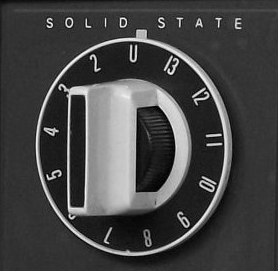
\includegraphics[width=35mm,bb=0 0 279 272]{figures/9bd96506bdaac48b26c5cd192851c11d.png}
   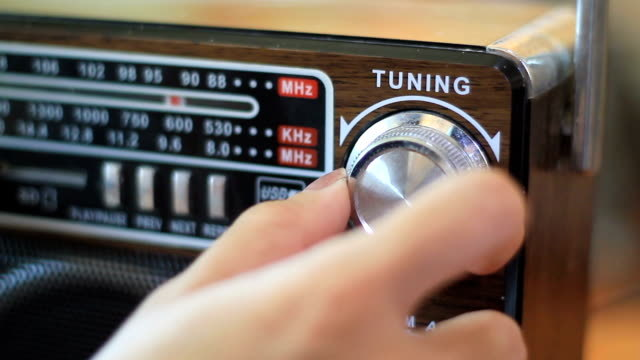
\includegraphics[width=35mm,bb=0 0 128 72]{figures/fedc4f3c899c48b5a3ddd0982801c79d.png}
}
\caption{An old TV channel dial and a radio tuning dial}
\label{TV channel}
\end{figure}


% 一般に、選択するとすぐに見えるのはどこでも便利なものである
% Finderのカバーフローや、最下層では選択内容がすぐに見えたりする
% このときはConfirmの手間なく内容を見られるのは便利なもので、
% これをno-click browsingと呼ぶことにする
% TVもラジオもno-click browsingが可能であった

It is always convenient to view the contents of the selected item
as soon as we find it.
We call such viewing style as ``\textbf{\tit{no-click browsing}}''.

We can use the no-click browsing style on personal computers.
Using the Finder.app on MacOS, we can use the ``Cover Flow''\footnote{
  \tsf{https://en.wikipedia.org/wiki/Cover\_Flow}
} viewer to browse the contents in a folder
with simple swiping gestures (Figure \ref{coverflow}).

\begin{figure}[H]
\centerline{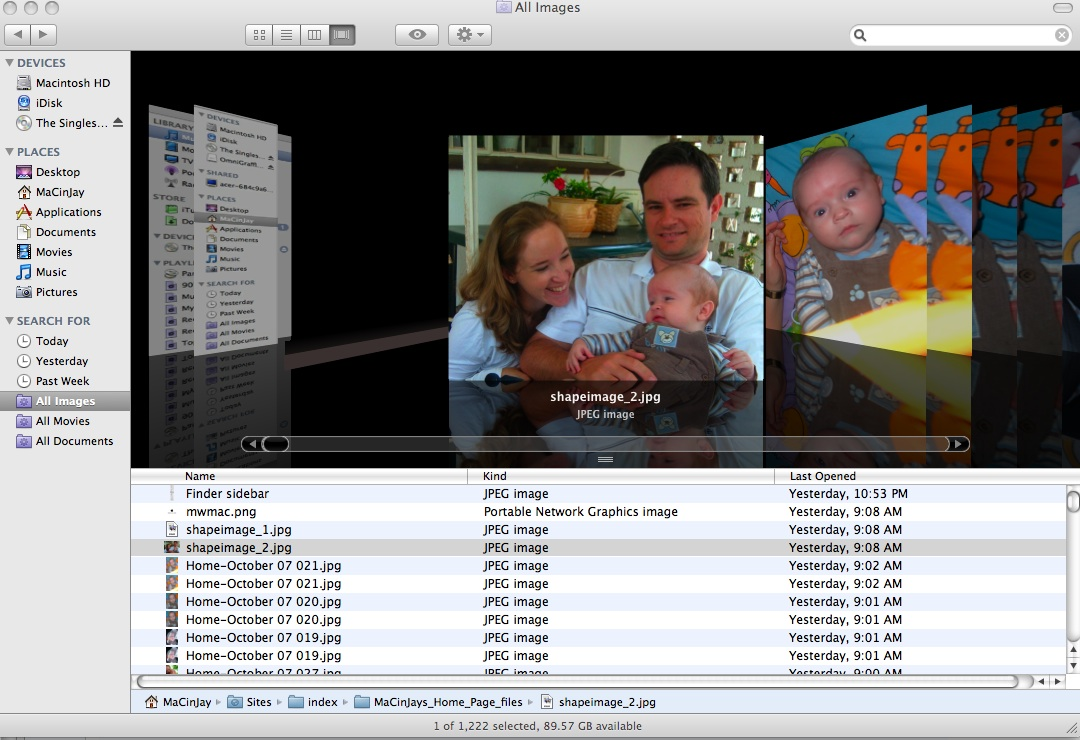
\includegraphics[width=65mm,bb=0 0 1080 740]{figures/902678c6770b5e043baa6f503375749f.jpg}}
% \centerline{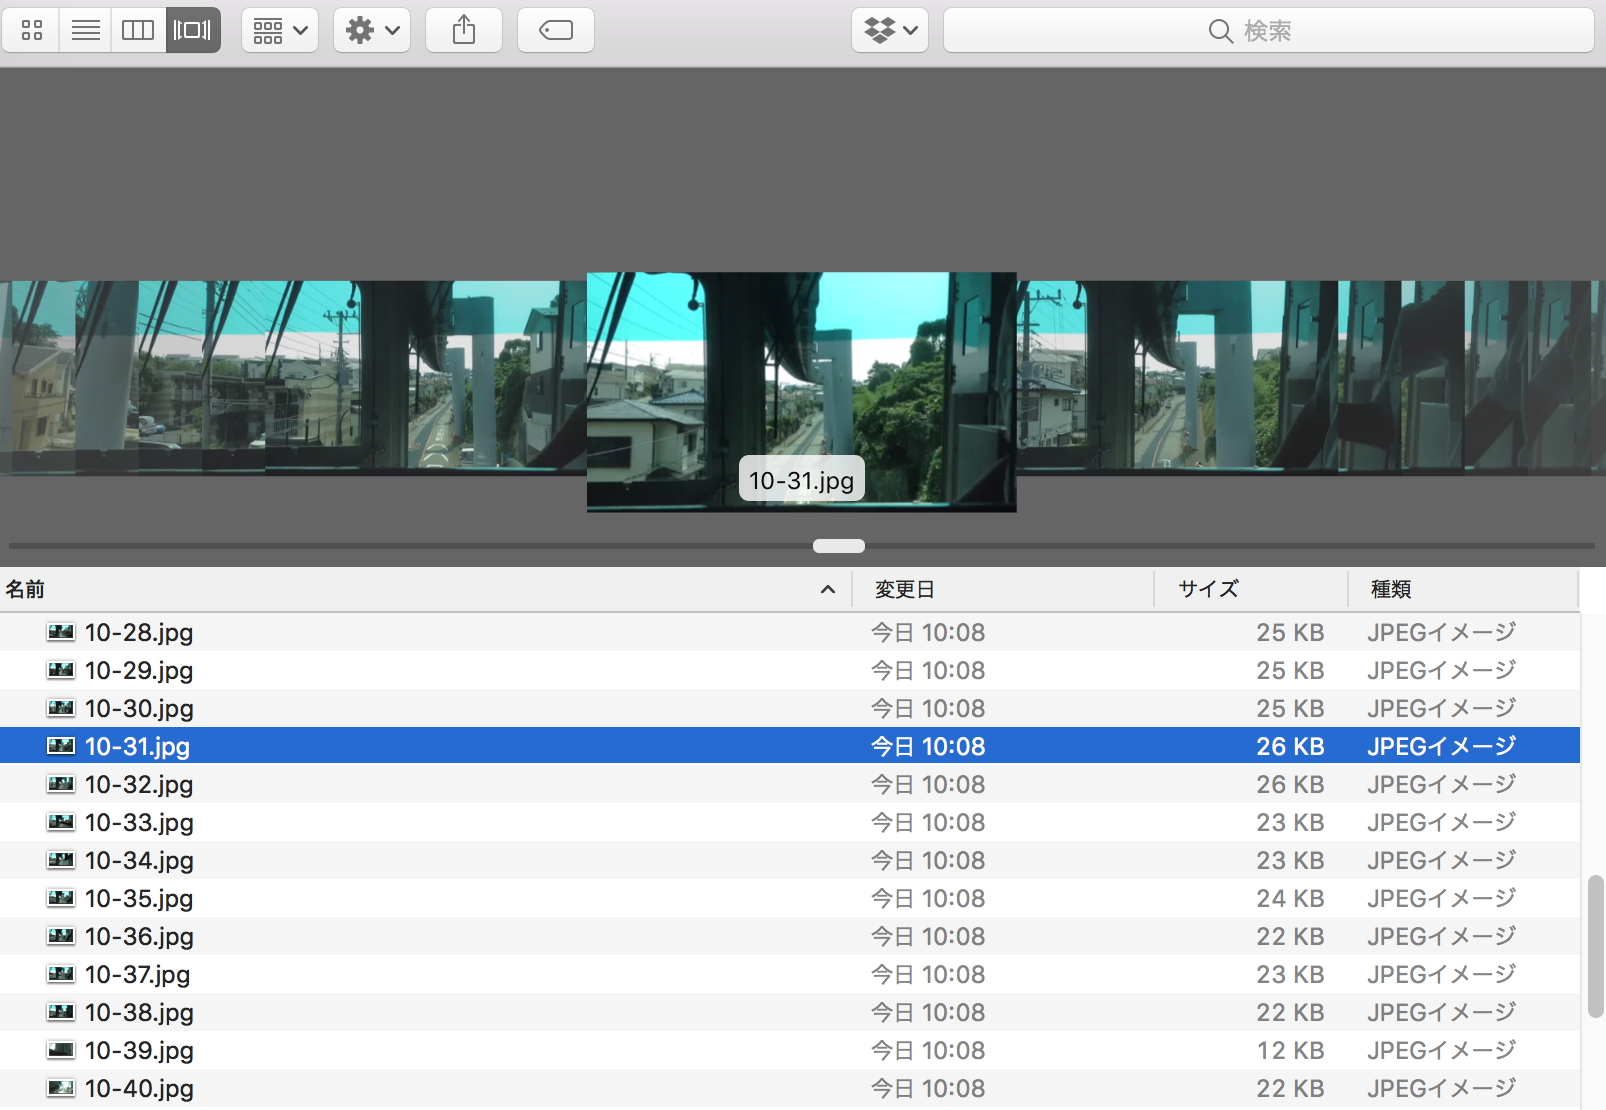
\includegraphics[width=80mm,bb=0 0 803 555]{figures/5d46fb09c3c5b4baccfd68ca026ef25b.png}} % Monorail
\caption{Cover Flow on MacOS}
\label{coverflow}
\end{figure}

We can also enjoy no-click browsing on the ``column view'' mode of Finder.app.
In the column view mode, 
the contents of the file is shown at the right side of the window
as soon as we select a file in a folder (Figure \ref{noclickfinder}).
When we type an arrow key and select another file,
the contents is shown instantly without a confirm operation.

\begin{figure}[H]
% \centerline{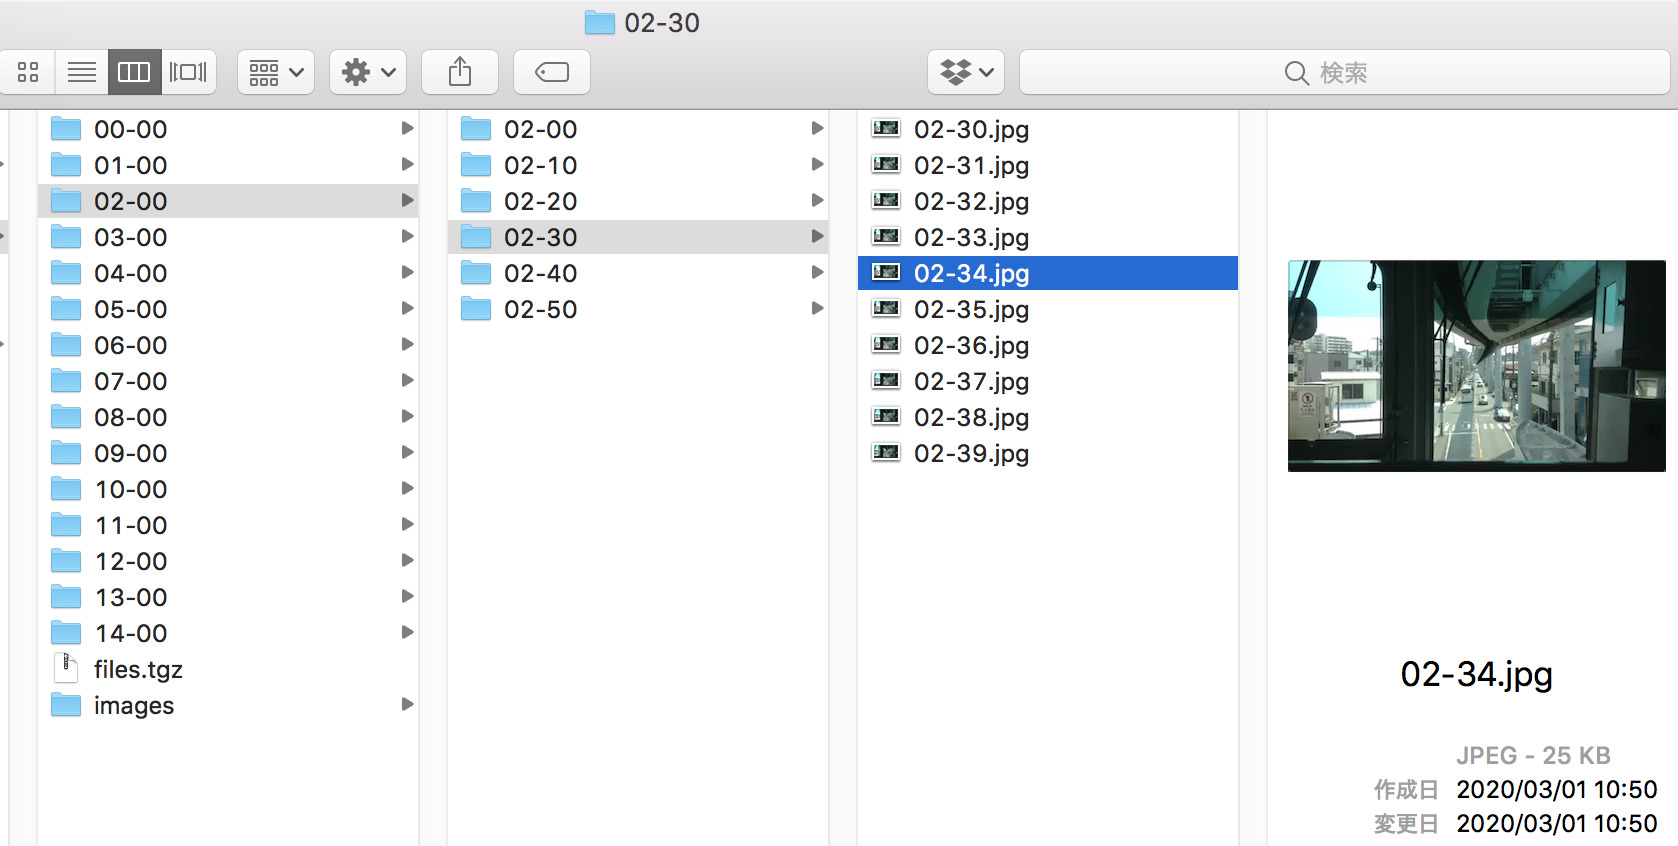
\includegraphics[width=70mm,bb=0 0 1678 846]{figures/10d7ca6c55aa93ebcdab799246e4c087.jpg}}
\centerline{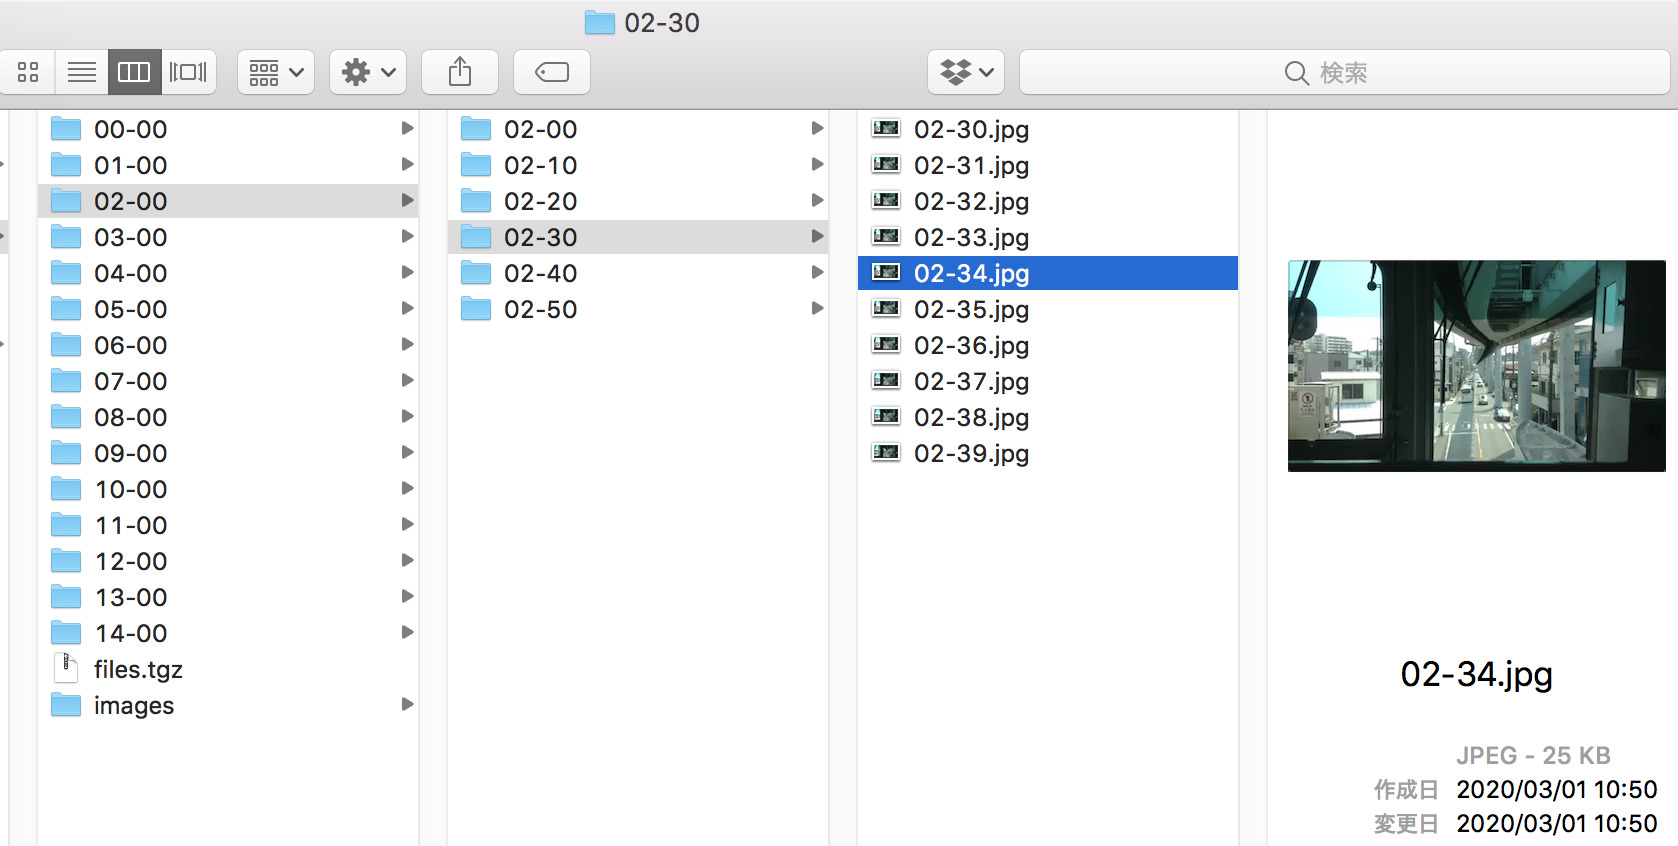
\includegraphics[width=70mm,bb=0 0 839 423]{figures/10d7ca6c55aa93ebcdab799246e4c087.jpg}}
\caption{No-click browsing on the ``column view'' of Finder.app.}
\label{noclickfinder}
\end{figure}


% テレビやカバーフローのザッピングはもちろんソースが少なかったからできるわけだが、
% 大量データの場合はこれが難しい。
% 何千個もソースがある場合は
% 階層をたどる処理が必要になり、その移動操作が必要だからである

We can use no-click browsing on old TVs and radios because the number of
broadcast channels are limited.
Likewise, no-click browsing on Finder.app is useful
when the number of files in a folder is not very large.

No-click browsing is not popular on conventional GUI of personal computers.
People are used to click-based browsing on web browsers and other
information visualization systems.
People can navigate through a huge information space by
clicking links, zooming by dragging, and using other GUI techniques.
These techniques are useful for finding an item in a large information space,
but many clicks and drag operations are required,
and the contents of the items are usually not shown during the search.

% 階層でもそうでなくても、移動操作は慣れている
% 適切な階層構造を用意して、クリックしながらたどるのがブラウザでは一般的である
% ブラウザの場合、カバーフローのようなインタフェースは一般的でないので、
% みつけたものを選択したり戻ったりを繰り返さなければならない。
% 
% ブラウザでは階層のInfoVis[]もいろいろあるが、操作に頭を使うし、no-clickブラウジングできるものは無い。

% 階層的なら上下操作でなんとかなる
% 小型機器で階層情報をたどるときは4-wayでひとつずつたどるのが普通

% The simplest way of navigatin a hierarchical data is to use four keys

When a user cannot use a pointing device,
key-based interaction techniques are used for
finding information in hierarchical data.
%
For example, a user can find a music data by
selecting an artist from the list of artist names,
selecting an album title from the title list,
and selecting a music title from the song list.
%
Users can use two keys for choosing an entry from the list
% (e.g. selecting an artist from the artist list),
and use another key for selecting an entry and moving to the next level.
% (e.g. selecting an artist and show album titles).
It is also necessary to use another key for going back to the previous level.
% (e.g. showing the artist list for artist selection).
This 4-way navigation is popular on small devices
and remote controllers for selecting a song from the hierarchical data.
4-way navigation is also available on the column view of Finder.app.

\begin{figure}[H]
\centerline{
  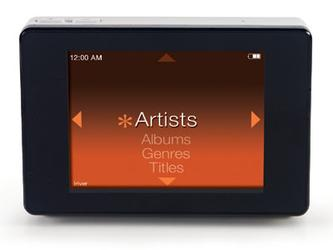
\includegraphics[width=30mm,bb=0 0 333 250]{figures/0048a5e91ddcf1d5670bd958e3c55619.jpg}
  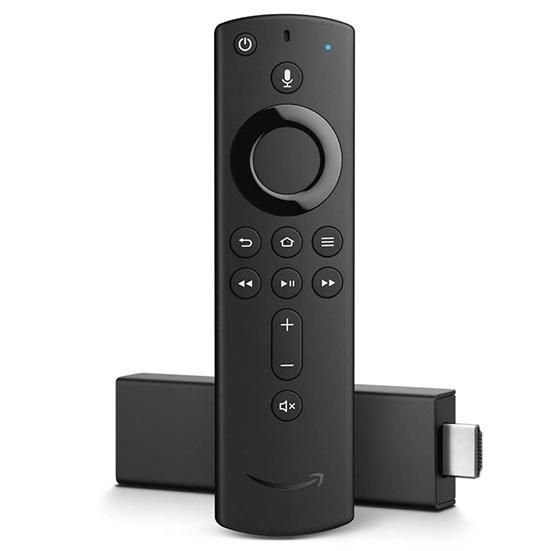
\includegraphics[width=30mm,bb=0 0 551 551]{figures/70c036b24525c6cace9955b24152e97e.jpg}
  }
\caption{Small devices supporting 4-way navigation}
\label{rio}
\end{figure}

Using 4 keys might be okay on these devices, but it would be better
if we could perform the navigation task using simpler devices that have only two keys.
In that case, we can use a rotating device like a disk or a wheel for the navigation,
since such devices can generate two signals based on the rotation direction.

We have developed a new navigation technique called ``{Gear}'' for no-click browsing,
where users can explore a large hierarchical database by using only two keys.


\section{Navigation method of Gear}
\label{navigation}

Interaction with Gear is based on the following simple principles.
Two types of operations,
{\up} (up) and {\down} (down), are used for the navigation.
They can be performed either by pressing keys or rotating a dial.

\begin{enumerate}
\item A portion of hierarchical data is shown to the user as a list.

\item One element in the list is selected and highlighted.

% \item Display the selected element, its siblings, its ancestors and their siblings.

\item When an element is selected, its siblings, its ancestors and their siblings are displayed
around the selected element.

\item Users can issue {\up} to select the element above the currently selected element,
or issue {\down} to select the element below the selected element.
Whenever the selection is changed, 3. is performed.
If the depth of the newly selected element is different from the currently
selected element, siblings of the currently selected element disappear.

\item When a newly selected element has children and the user performs no further action,
the first child of the selected element is newly selected, and 3. is performed.
As a result, all the siblings of the newly selected element
(the first child of the currently selected element) appear in the list.

\end{enumerate}

We show how Gear works, using a hierarchical data structure of
a shops list in a shopping mall shown in Figure \ref{fig1} as example data.
A rectangles with a thick border represent shop categories, and
other rectangles represent individual shops.

\begin{figure}[H]
% 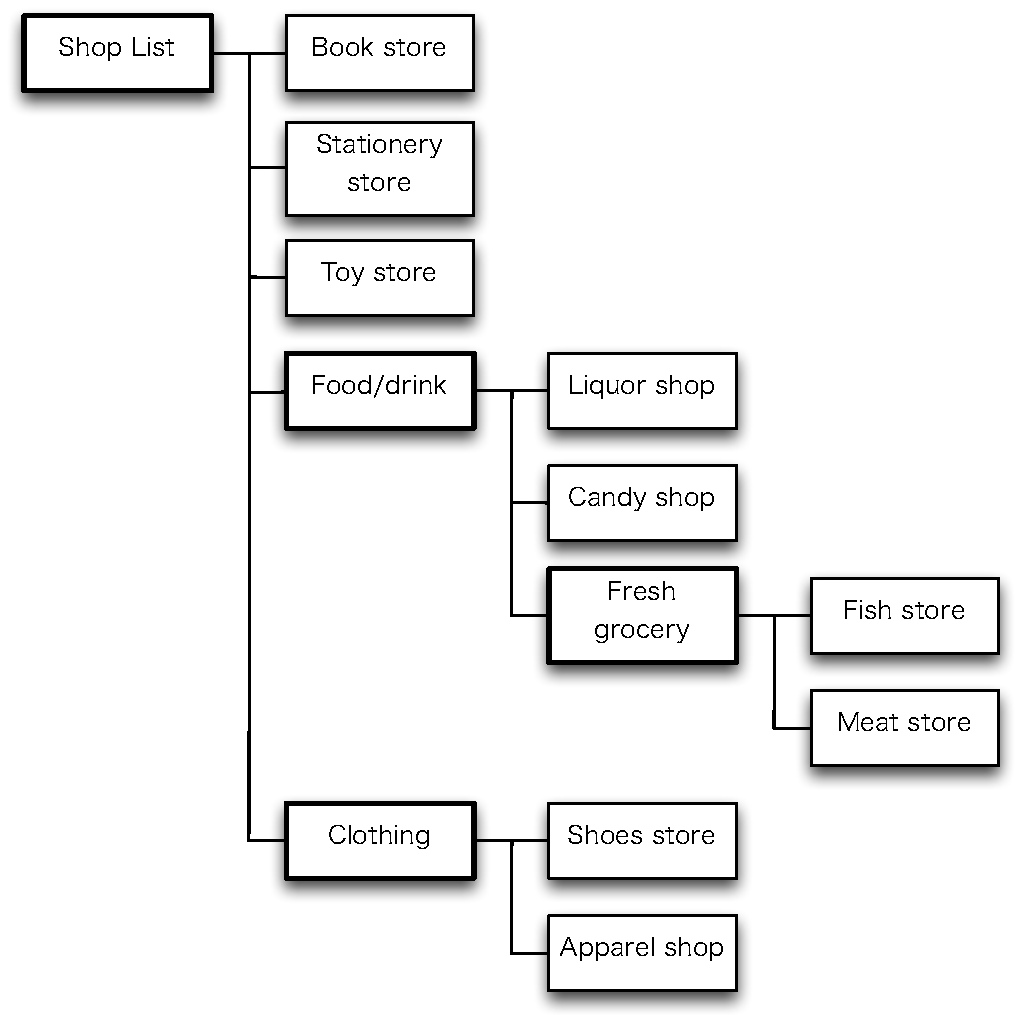
\includegraphics[width=70mm]{figures/fig1.pdf}
\centerline{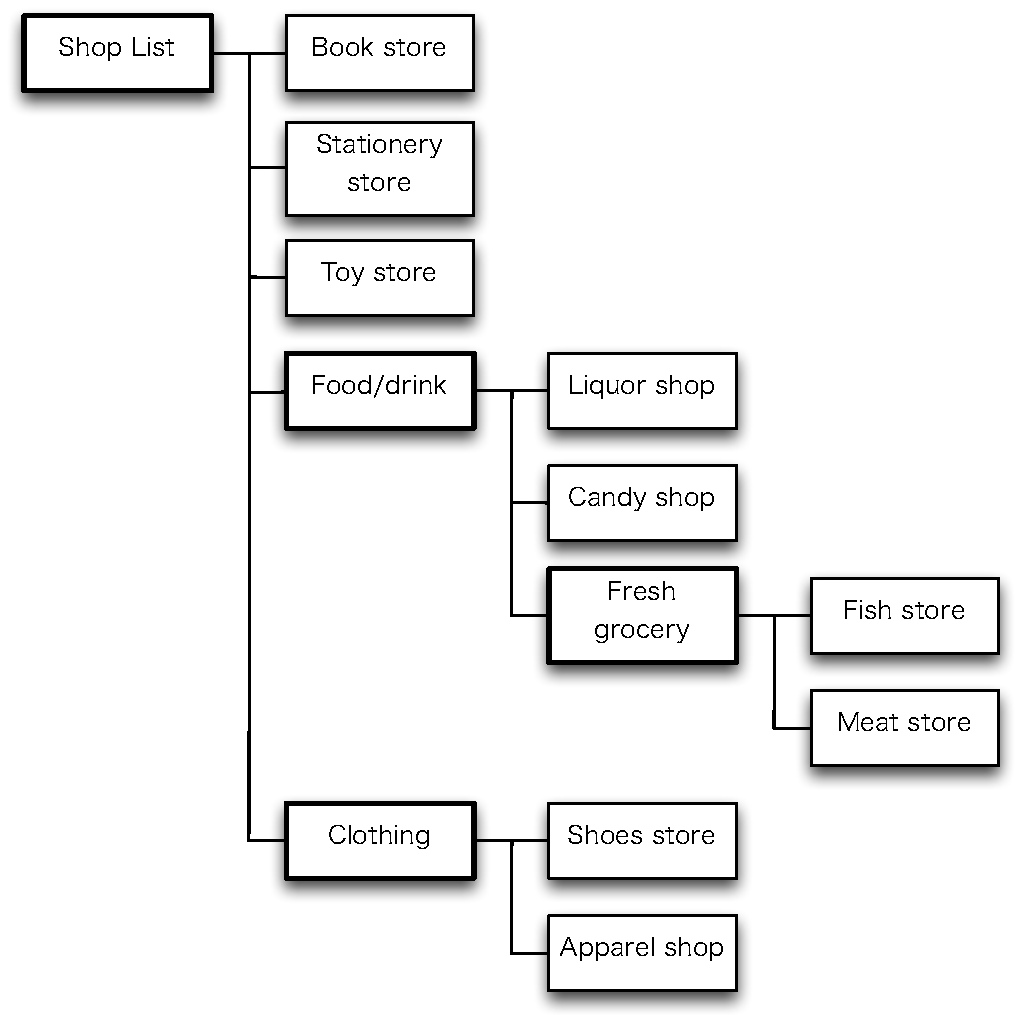
\includegraphics[width=70mm,bb=0 0 490 490]{figures/fig1.pdf}}
\caption{Sample data: shops data of a shopping mall.}
\label{fig1}
\end{figure}

When a user starts the exploration, only the shops and categories
at the top level are displayed (Figure \ref{fig2}).
When the user issues {\down},
the second element (\tsf{Stationery store}) is selected (Figure \ref{fig3}).

\def\menuwidth{22mm}

\begin{figure}[H]
\centerline{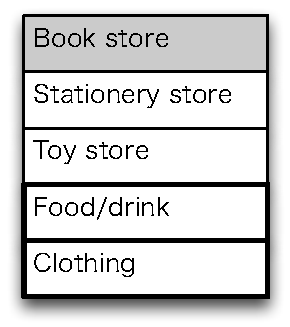
\includegraphics[width=\menuwidth, bb=0 0 139 157]{figures/fig2.pdf}}
\caption{Initial display.}
\label{fig2}
\end{figure}

\begin{figure}[H]
\centerline{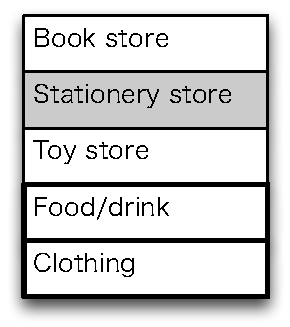
\includegraphics[width=\menuwidth,bb=0 0 139 157]{figures/fig3.pdf}}
\caption{Typing {\down}.}
\label{fig3}
\end{figure}

If the user issues {\down} two more times, 
\tsf{Food/drink} category is selected (Figure \ref{fig4}).
If the user stops the operation and waits for a moment, the shops under the \tsf{Food/drink}
category are automatically displayed,
and the first entry (\tsf{Liquor shop}) is selected (Figure \ref{fig5}).

\begin{figure}[H]
\centerline{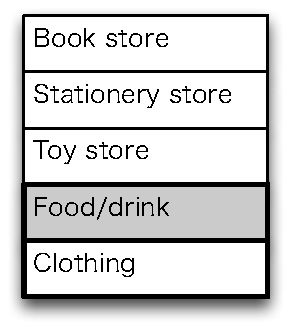
\includegraphics[width=\menuwidth,bb=0 0 139 157]{figures/fig4.pdf}}
\caption{Selecting Food/drink.}
\label{fig4}
\end{figure}

\begin{figure}[H]
\centerline{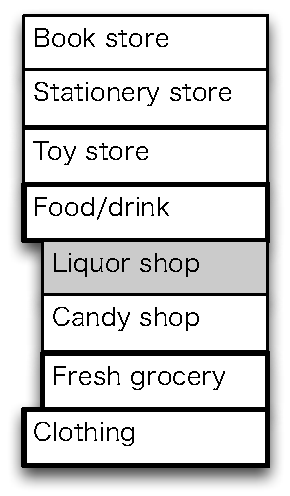
\includegraphics[width=\menuwidth,bb=0 0 139 238]{figures/fig5.pdf}}
\caption{Selecting Liquor shop.}
\label{fig5}
\end{figure}

When the user issues {\down} twice here,
\tsf{Fresh grocery} category is selected (Figure \ref{fig6}).

\begin{figure}[H]
\centerline{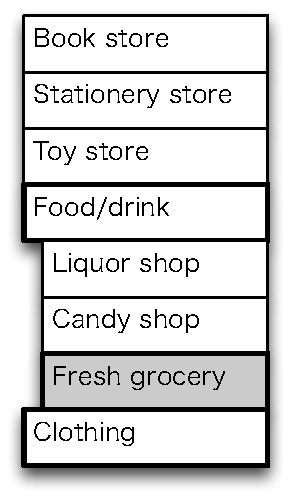
\includegraphics[width=\menuwidth,bb=0 0 139 238]{figures/fig6.pdf}}
\caption{Selecting Fresh grocery.}
\label{fig6}
\end{figure}

If the user keeps issuing {\down}, 
the list will change to Figure \ref{fig8},
without expanding the children of \tsf{Fresh grocery}.

\begin{figure}[H]
\centerline{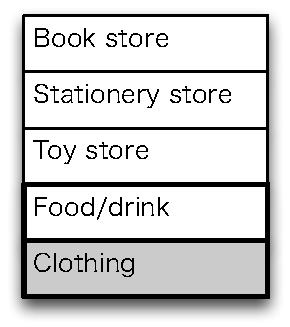
\includegraphics[width=\menuwidth,bb=0 0 139 157]{figures/fig8.pdf}}
\caption{Selecting Clothing.}
\label{fig8}
\end{figure}

If the use stops issuing {\down} at Figure \ref{fig6},
the shops under category \tsf{Fresh grocery} is automatically selected (Figure \ref{fig7}).

\begin{figure}[H]
\centerline{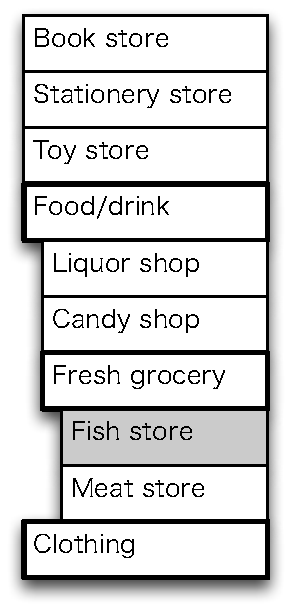
\includegraphics[width=\menuwidth,bb=0 0 139 292]{figures/fig7.pdf}}
\caption{Selecting Fish store.}
\label{fig7}
\end{figure}

When the user issues {\up} here, \tsf{Fresh grocery} is selected,
and the shops under \tsf{Fresh grocery} disappears, 
resulting in the same state as Figure \ref{fig6}.
If the user issues {\up} two more times, the display changes to the state
shown in Figure \ref{fig5},
and one more {\up} will set the system to the state of Figure \ref{fig4}.

If the user issues {\down} in Figure \ref{fig4}, the next visible entry
(\tsf{Clothing}) is selected (Figure \ref{fig8}), and then the state changes to Figure \ref{fig9}.

\begin{figure}[H]
\centerline{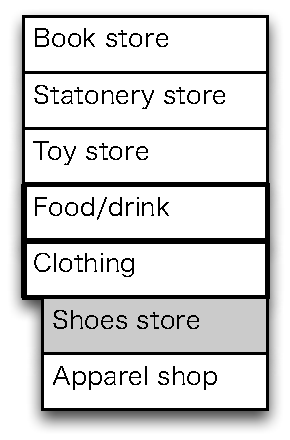
\includegraphics[width=\menuwidth,bb=0 0 139 211]{figures/fig9.pdf}}
\caption{Selecting Shoes store.}
\label{fig9}
\end{figure}

When the user issues {\down} twice in Figure \ref{fig7},
\tsf{Clothing} is selected, and the category under \tsf{Food/drink} will shrink (Figure \ref{fig8}).

In this way, users can explore the hierarchical structure
only by issuing {\up} and {\down} at the right timing.

\section{Serencast: a no-click browsing service}

% SerencastというサービスでGearを使う
% SerencastはScrapboxを利用したものである

To prove that Gear is useful for selecting an entry from a
large hierarchical database,
we have developed the ``\tsf{\SC}'' service, where
users can enjoy movies, musics, and other web services
on the browser with the Gear interface without selecting (clicking) an item.
{\SC} is implemented in JavaScript, and runs on modern web browsers

{\SC} uses the ``\tsf{\SB}'' wiki service\footnote{
  \tsf{https://Scrapbox.io/}
} for listing the contents of the hierarchical database.
{\SB} is an interactive wiki
system where users can share and edit texts on the web browser.
A user can create a {\SB} ``project'', and create pages
that consists of texts and links.
People can share the page and edit it interactively on their browsers
just like the Google Docs system\footnote{
  \tsf{https://www.google.com/docs/about/}
}.

\begin{figure}[H]
\centerline{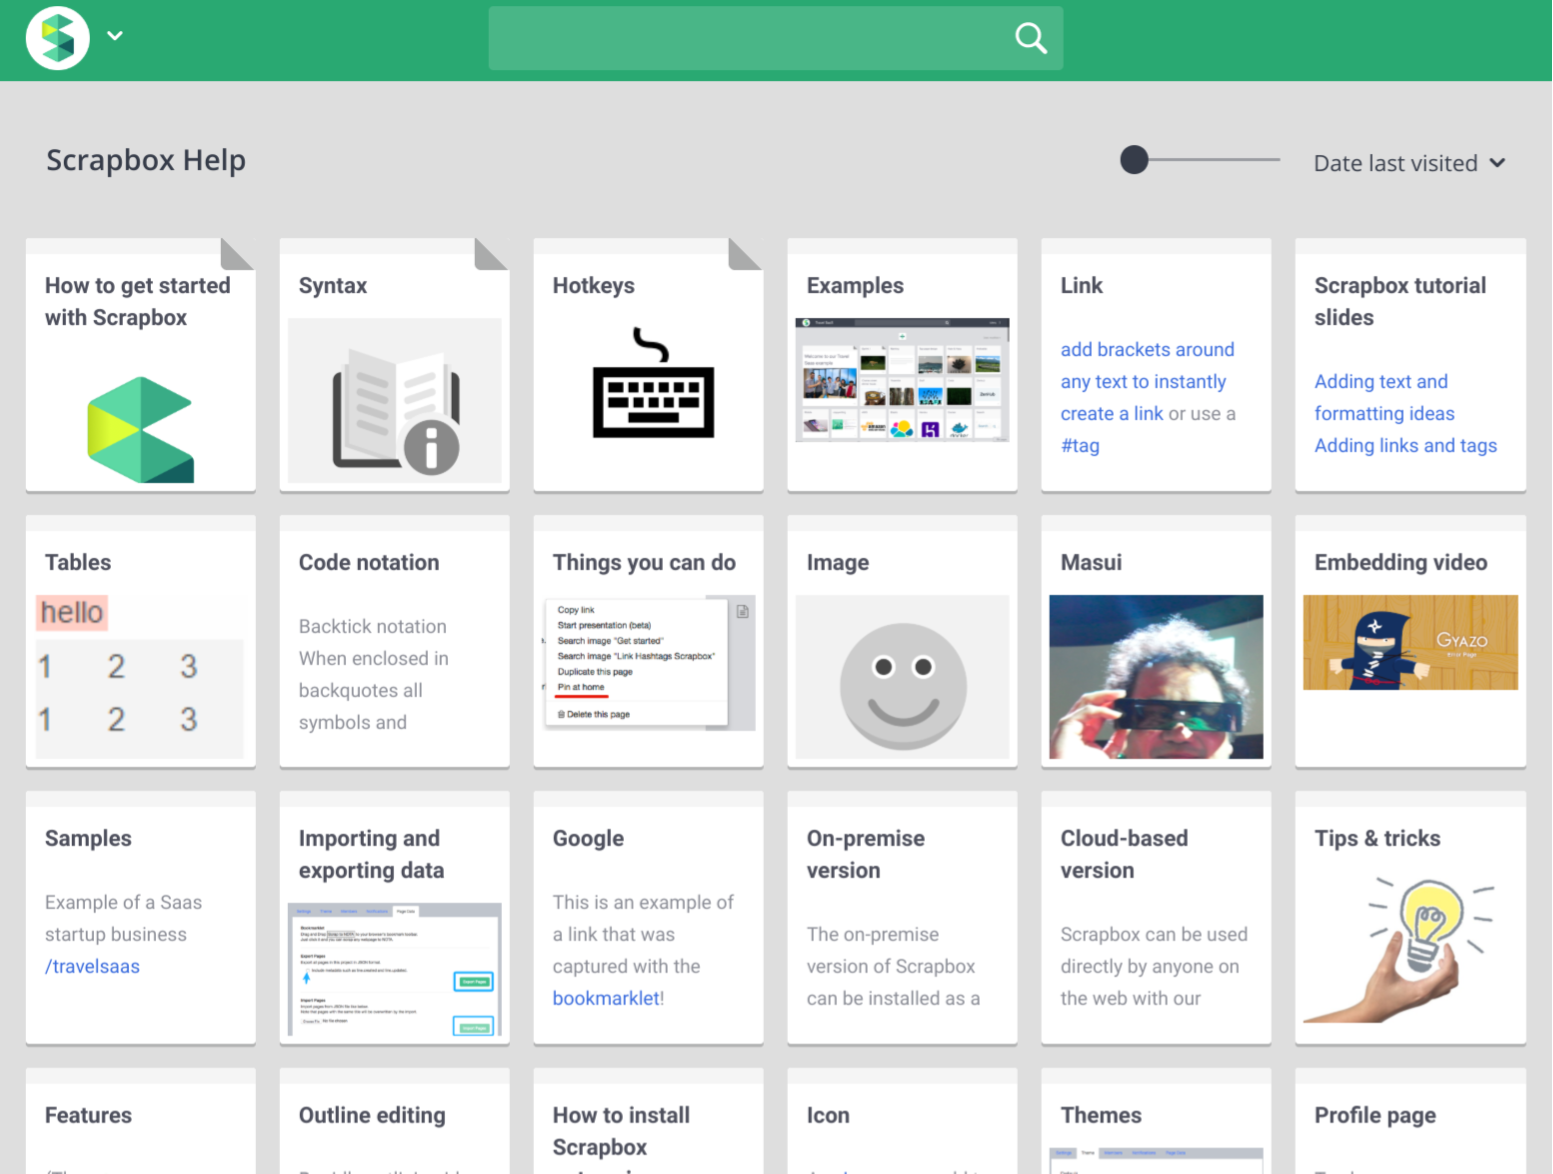
\includegraphics[width=75mm,bb=0 0 1553 1174]{figures/28818d749896f87f3eb8bd6b6f9e9a36.png}}
\caption{An example of a {\SB} project.}
\label{exampleproject}
\end{figure}

Figure \ref{exampleproject} shows an example of a {\SB} project.
The title of the project is ``Scrapbox help'', and
other pages like ``Features'' exist in the project.

\begin{figure}[H]
\centerline{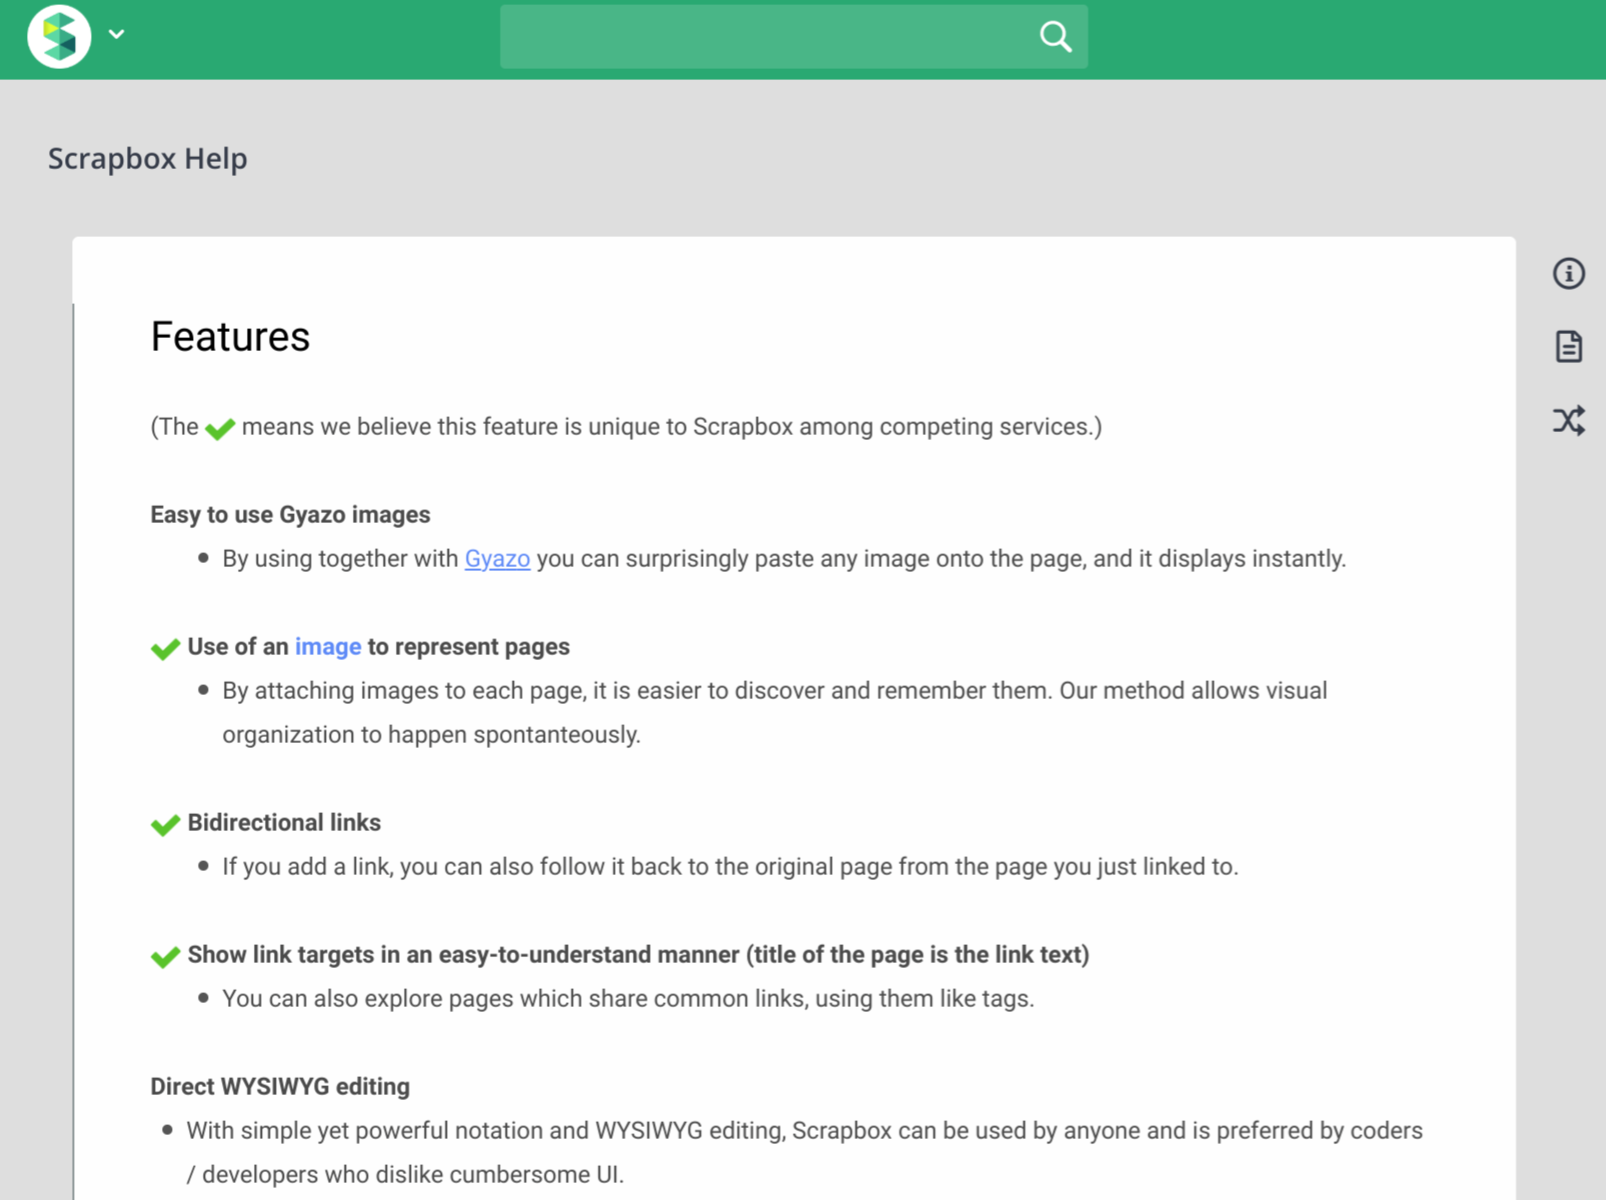
\includegraphics[width=80mm,bb=0 0 1606 1200]{figures/9e867c325bafc415bd0870c1717fbaf7.png}}
\caption{An example {\SB} page.}
\label{examplepage}
\end{figure}

Figure \ref{examplepage} is an example of a {\SB} page.
%
The page is based on plain text just like an WikiPedia page is based on plain text.
Users can use special markup tags
like ``\texttt{[}'' and ``\texttt{]}'' to show bold texts, icons, URL links,
and links to other pages.
In this example, a URL link to {\tsf{http://gyazo.com}} is used
just like an \tsf{A} tags in HTML.

The raw text of the {\SB} page looks like this:

{\scriptsize
\begin{verbatim}
Features
(The [Check.icon] means we believe this feature is unique \
 to {\SB} among competing services.)

[[Easy to use Gyazo images]]
 By using together with [Gyazo https://gyazo.com] you can \
 surprisingly paste any image onto the page, and it \
 displays instantly.

[Check.icon] [[Use of an [image] to represent pages]]
 By attaching images to each page, it is easier to discover \
and remember them. Our method allows visual organization to \
happen spontanteously.
\end{verbatim}
}

When we list the URLs of Web pages of
movies and musics on a {\SB} page,
% we can create a hierarchical structure from the list and
% use the Gear interface to find data and browse it.
We can use {\SC} service
for using the Gear interface to select a program from the
list on {\SC} pages, and automatically play it on the browser.

Figure \ref{movielist} shows the movie list defined in a {\SB} page.

\begin{figure}[H]
% \centerline{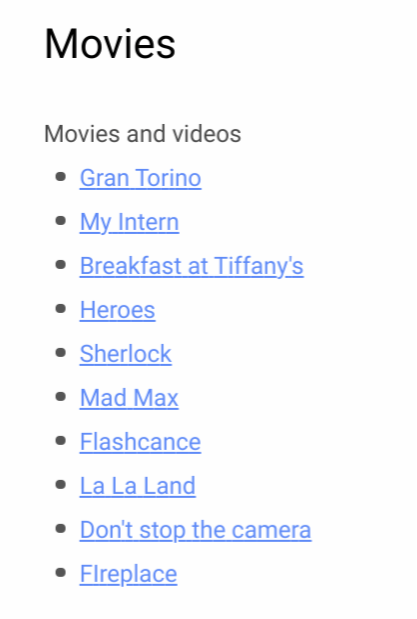
\includegraphics[width=40mm,bb=0 0 417 619]{figures/2690db244045aa809a3e2fc2b40ba0a3.png}}
\centerline{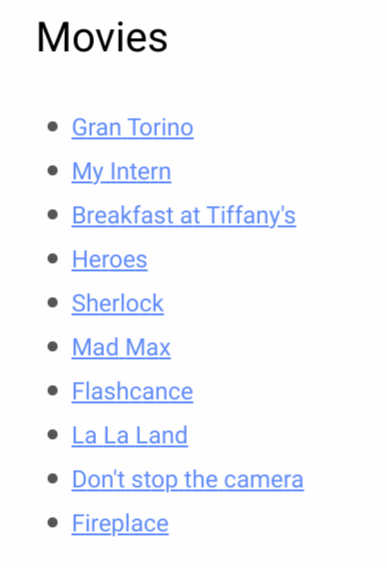
\includegraphics[width=30mm,bb=0 0 387 568]{figures/2b97930bf5730fcaf4d9c0adeb9c5f6e.png}}
\caption{A movie list page on {\SB}.}
\label{movielist}
\end{figure}

The raw text of this page is shown below:

{\scriptsize
\begin{verbatim}
Movies
 [https://www.netflix.com/watch/70105600 Gran Torino]
 [https://www.netflix.com/watch/80047616 My Intern]
 [https://www.netflix.com/watch/330201 Breakfast at Tiffany's]
 [https://www.netflix.com/watch/70080178 Heroes]
 [https://www.netflix.com/watch/70174781 Sherlock]
 [https://www.happyon.jp/watch/100048550 Mad Max]
 [https://www.netflix.com/watch/60010351 Flashdance]
 [https://www.netflix.com/watch/80095365 La La Land]
 [https://www.netflix.com/watch/81191988 Don't stop the camera]
 [https://youtube.com/embed/AtZr9g2vwrI?autoplay=1 Fireplace]
\end{verbatim}}

\begin{figure}[H]
% \centerline{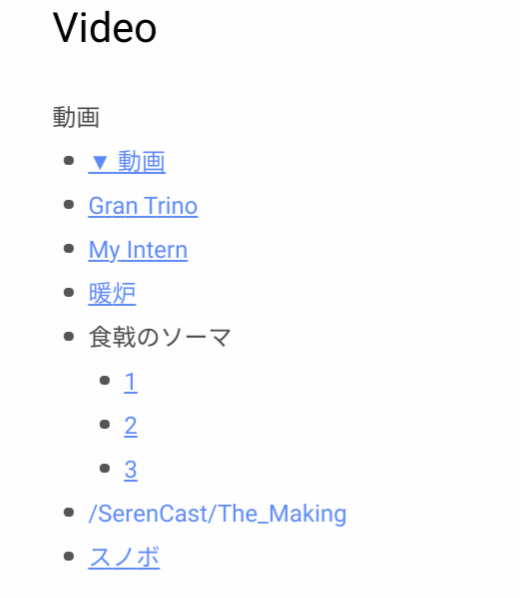
\includegraphics[width=80mm,bb=0 0 524 598]{figures/65b01a87b67c9a8e838a047b945f6a77.png}}
\centerline{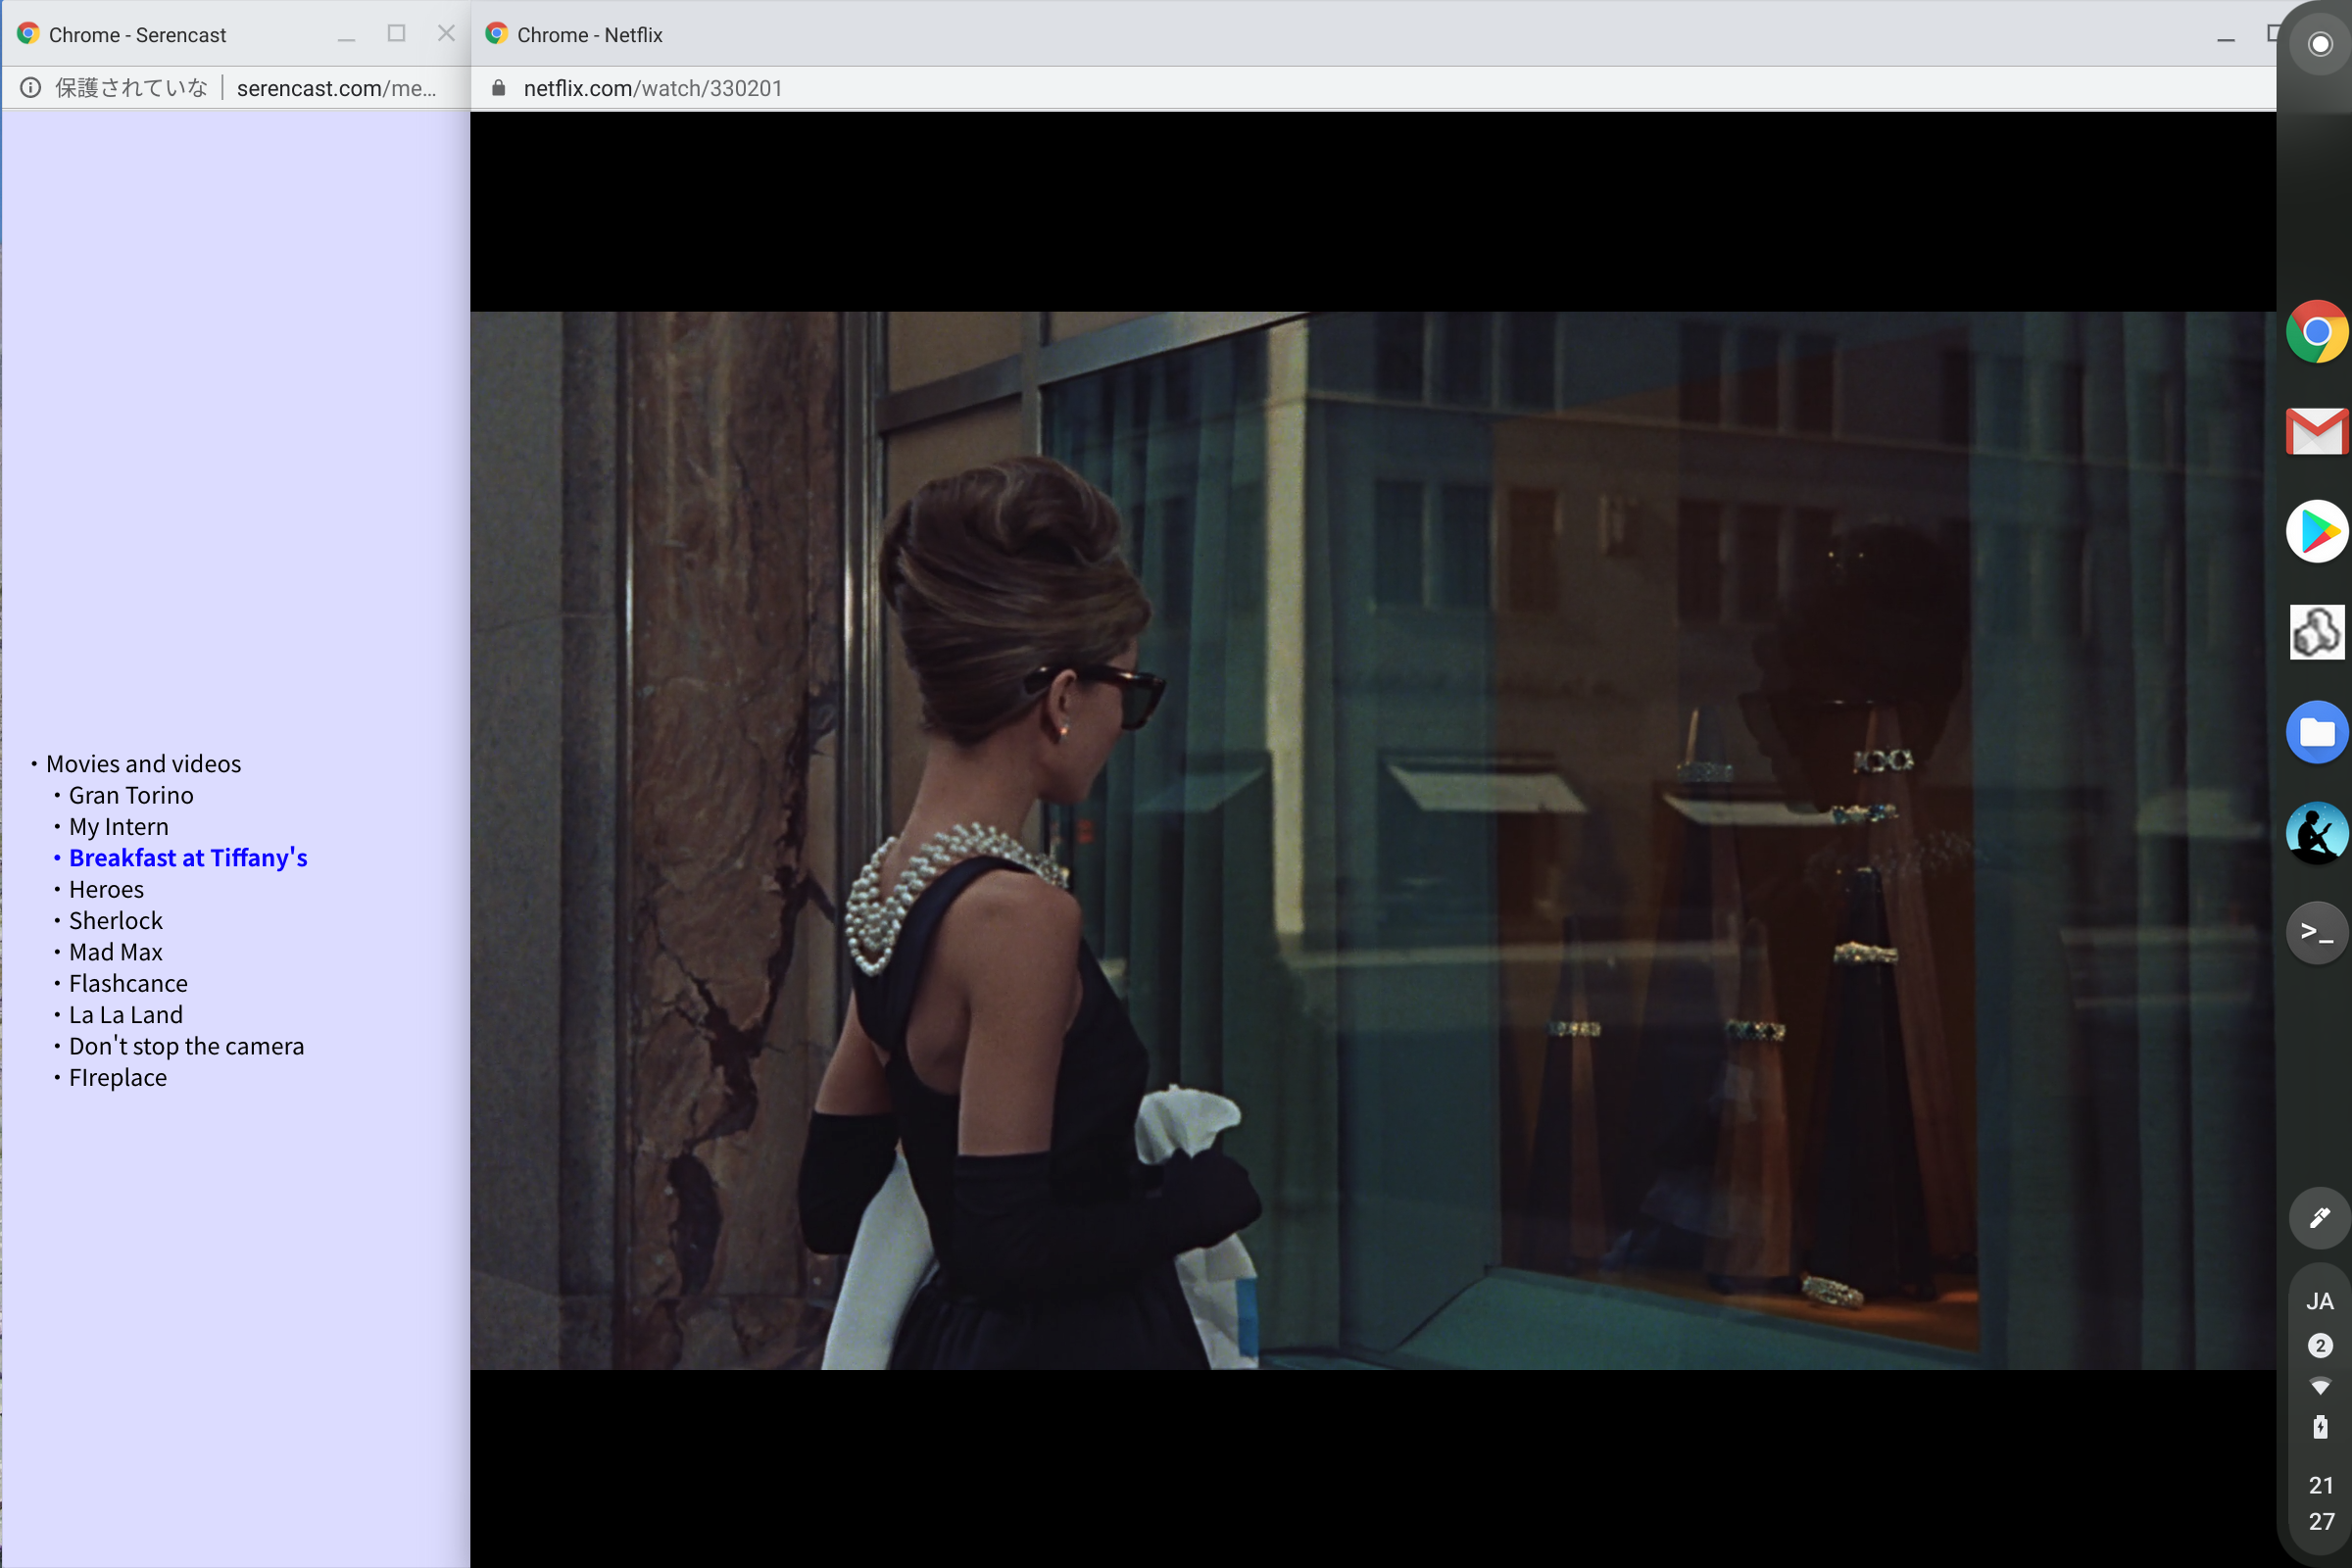
\includegraphics[width=80mm,bb=0 0 2400 1600]{figures/e8ae562a5a68a1955ac70b4faed9a146.png}}
\caption{Watching ``Breakfast at Tiffany's''.}
\label{tiffany}
\end{figure}

When we access this {\SB} page from {\SC},
``Gran Trino'' from Netflix automatically starts in the right side of the screen,
just like a TV program starts when we rotate the channel dial of an old television.
When the user pushes the {\down} key twice,
``Breakfast at Tiffarny's'' is selected and
the movie starts at the right side of the screen. (Figure \ref{tiffany})

In the above example, we can select only one of the 10 movies from the movie list.
But we can add more data by hierarchically providing contents in {\SB} pages.

In one page, we can specify a hierarchical structure by using indentations.
Figure \ref{musiclist} shows a portion of a list of music CDs and
titles by ``Weather Report'' and ``Wes Montgomery'' are shown\footnote{
  Weather Report is the name of a famous Jazz group, and Wes Montgomery is a famous Jazz guitarist.
}.
For example, 
``Black Market'' is the first title in the album ``8:30'' of ``Weather Report'', and
``Scarlet Woman'' follows ``Black Market''.
``Wes Montgomery'' is listed in the same layer as ``Weather Report'', and
the album ``Tequilla'' is listed one level below the level of the name of the artist.

\begin{figure}[H]
% \centerline{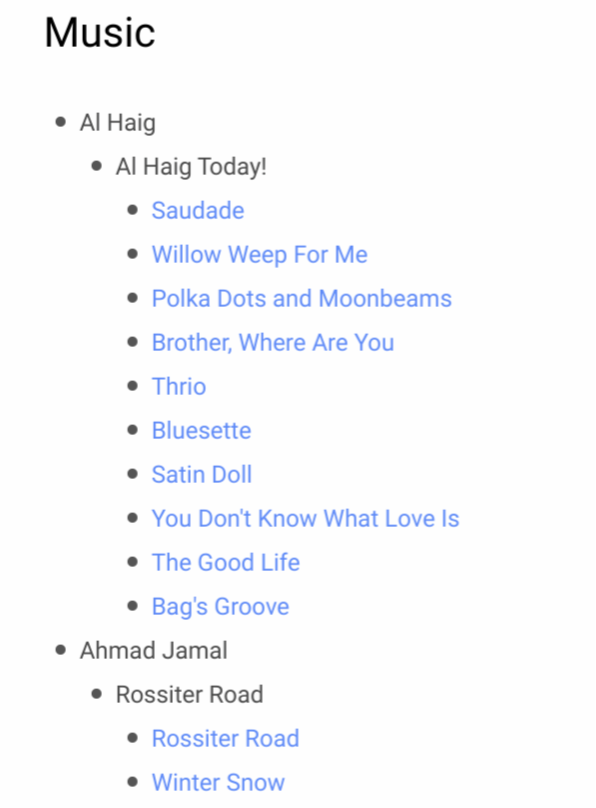
\includegraphics[width=40mm,bb=0 0 596 808]{figures/6657544cf60cbf0aea91ba7da0455b90.png}}
\centerline{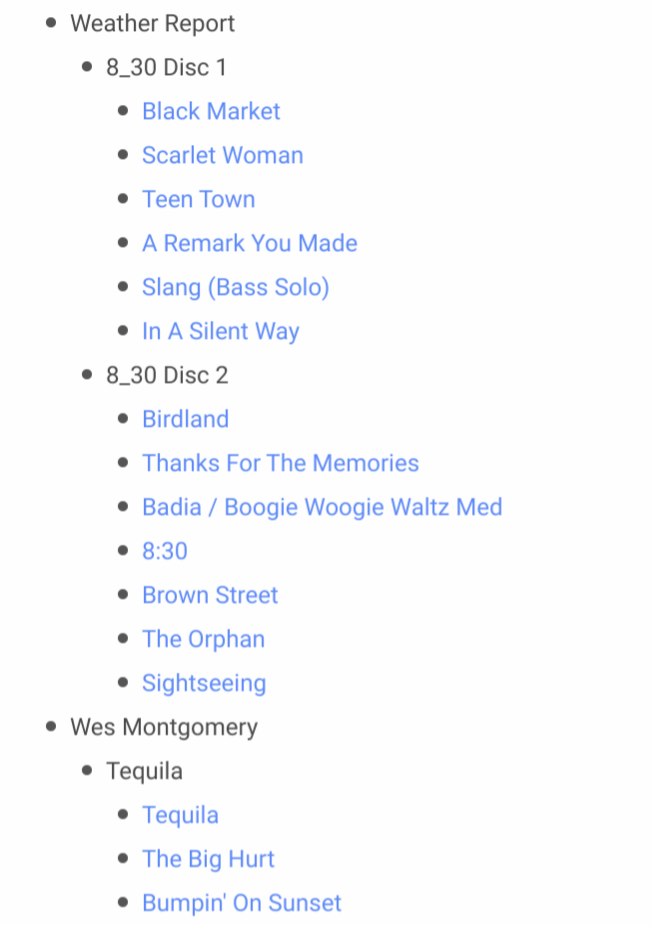
\includegraphics[width=50mm,bb=0 0 652 926]{figures/d8fe8ff8f3e1bbcb34cf51e268592f8c.png}}
\caption{Music list.}
\label{musiclist}
\end{figure}

The title of this {\SB} page is ``Music'', and 
we can collect Movie page, Music page, and other pages by
listing them in another page (``Top'' page, in this case).

\begin{figure}[H]
% \centerline{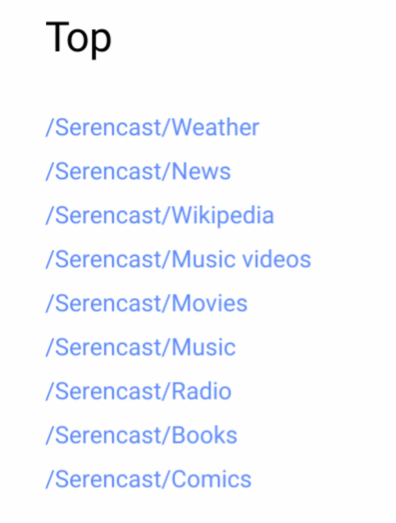
\includegraphics[width=40mm,bb=0 0 396 523]{figures/8a8e4d63b75183f1b4d0ed4db733f500.png}}
\centerline{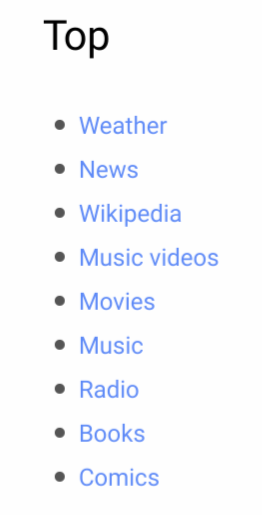
\includegraphics[width=27mm,bb=0 0 262 515]{figures/5a644f357ba6a6b81b011e200019d736.png}}
\caption{Top page.}
\label{top}
\end{figure}

Many pages (Music, Movies, etc.) are listed in the Top page, and
the pages are treated as children pages of the Top page.
By constructing data hierarchically like this,
We can build a very large hierarchical database for watching movies, videos, news, etc.
A hierarchical database with
As many as 100,000 pages can be easily constructed on a {\SB} pages, and
we can select one of the entries only by using only {\up} and {\down} keys,
using the Gear technique described in section \ref{navigation}.

\begin{figure}[H]
\centerline{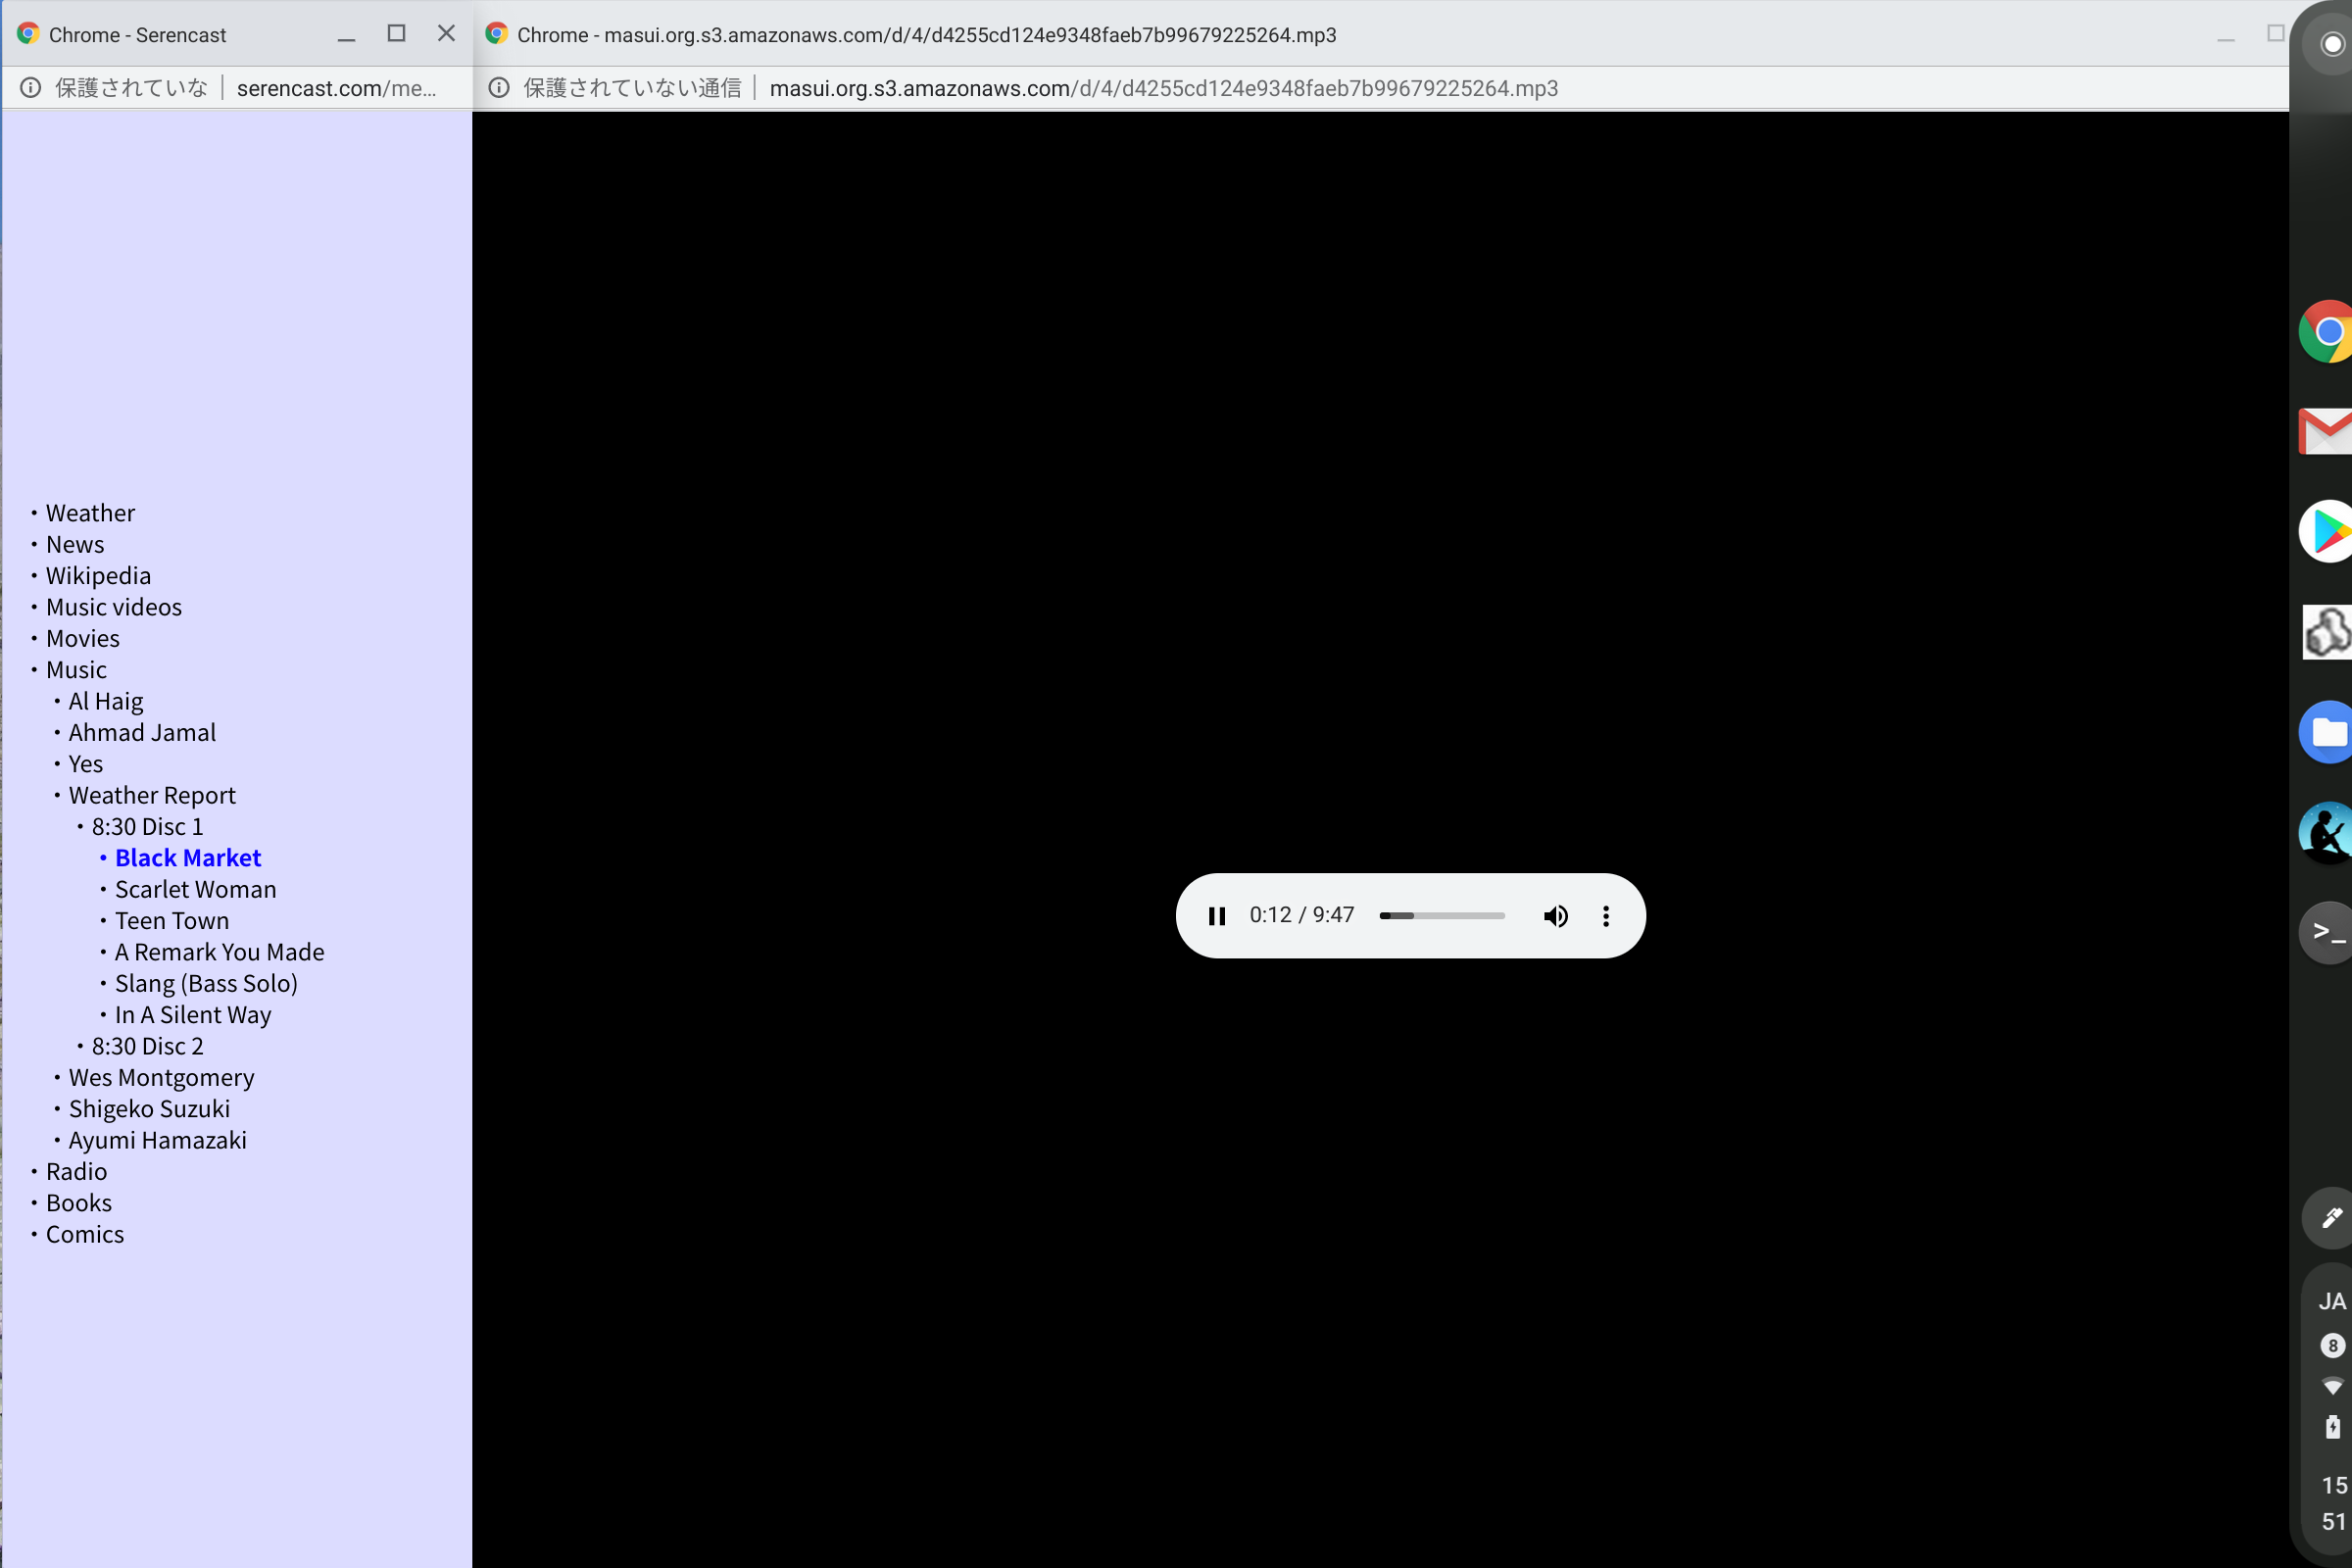
\includegraphics[width=80mm,bb=0 0 2400 1600]{figures/blackmarket.png}}
\caption{Playing a music.}
\label{blackmarket}
\end{figure}

\begin{figure}[H]
\centerline{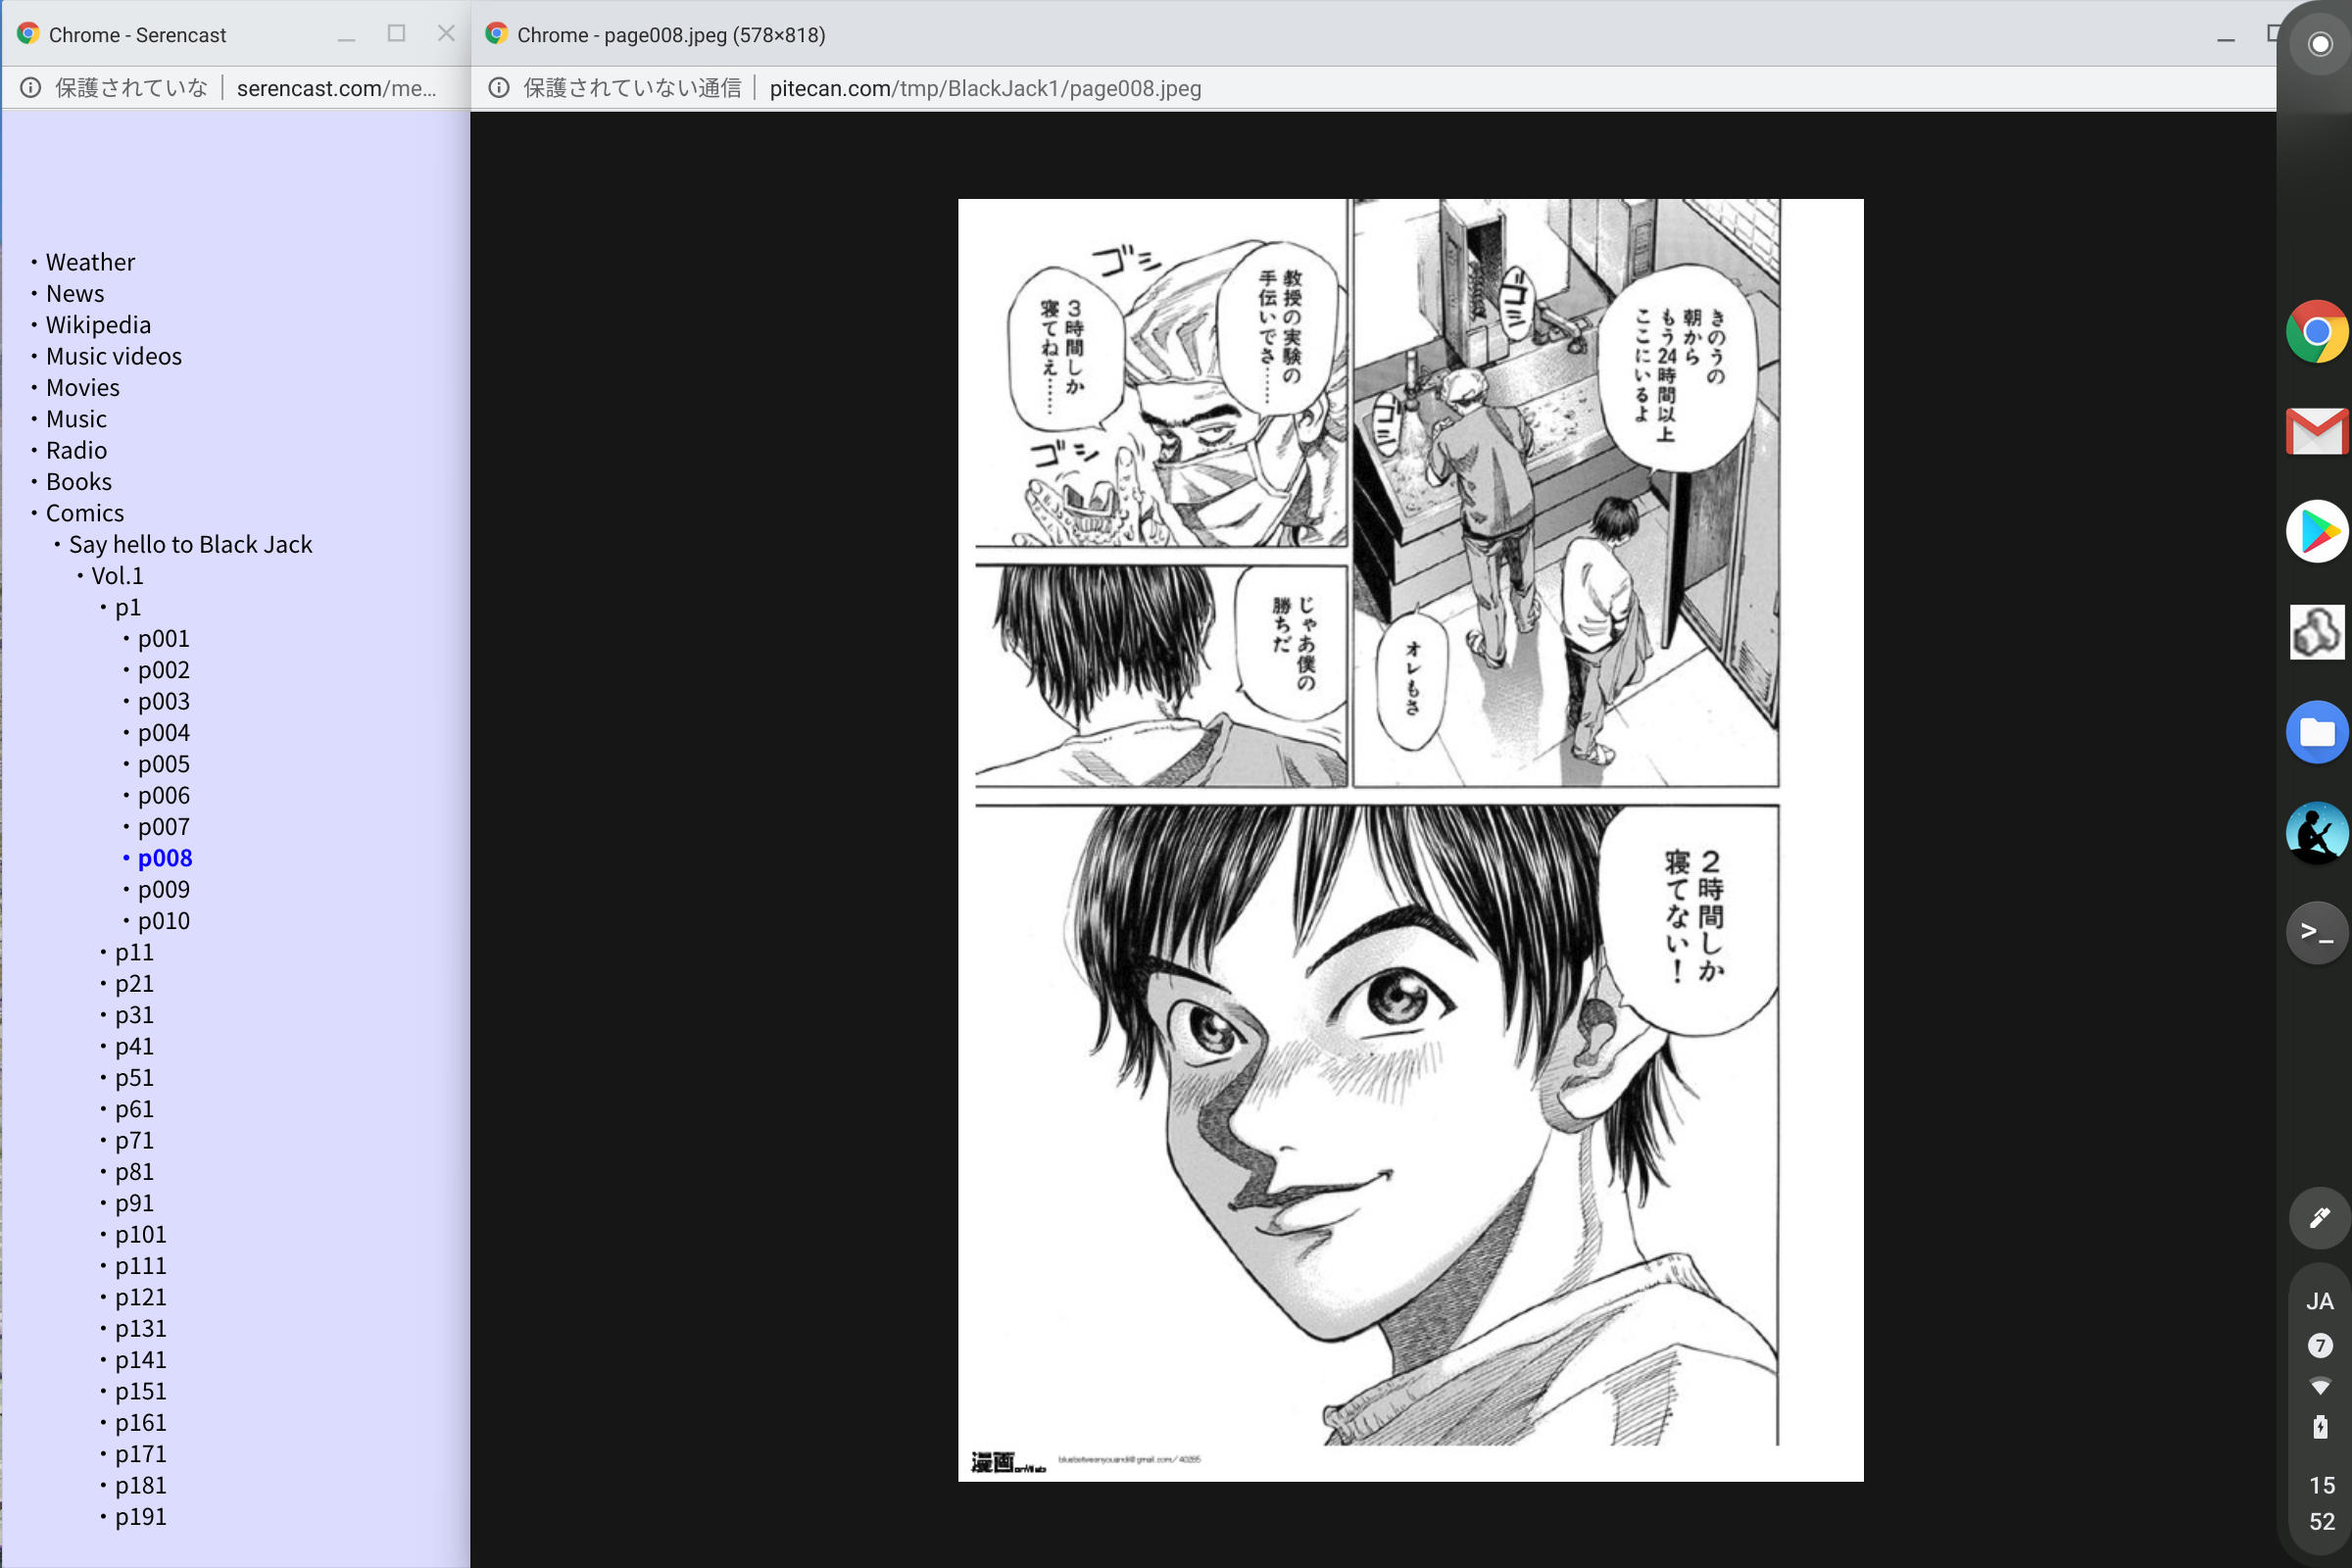
\includegraphics[width=80mm,bb=0 0 2400 1600]{figures/blackjack.png}}
\caption{Reading a comic book.}
\label{blackjack}
\end{figure}

Since anybody can edit {\SB} pages and construct the hierarchical data,
people can enjoy creating their own hierarchical database by editing their {\SB} pages.
When someone wants to advertise their works,
he can create his {\SB} pages
and give them to other people so that they can watch the pages.
People can freely include other people's {\SB} pages in their own list
and enjoy all the contents just by using Gear.

\section{Discussion}

\subsection{Input devices for Gear}

Since only two switches are required in the Gear interface,
almost any kind of input devices can be used for Gear.
We have tried various input devices and collected experiences.

\subsubsection{Keys and buttons}

The simplest input device for Gear may be keyboards and push buttons.
Gear works pretty comfortably with arrow keys on a PC.
Various HID devices\footnote{
  \tsf{https://en.wikipedia.org/wiki/Human\_interface\_device}
} are available on the market, and
all such devices can be used as an input device for Gear.
For example, a foot switch for turning music score pages\footnote{
  \tsf{https://airturn.com/products/airturn-pedpro}
} can be used as an input device for Gear.
Even a special foot pedal can be used for Gear (Figure \ref{footswitch}).

\begin{figure}[H]
\centerline{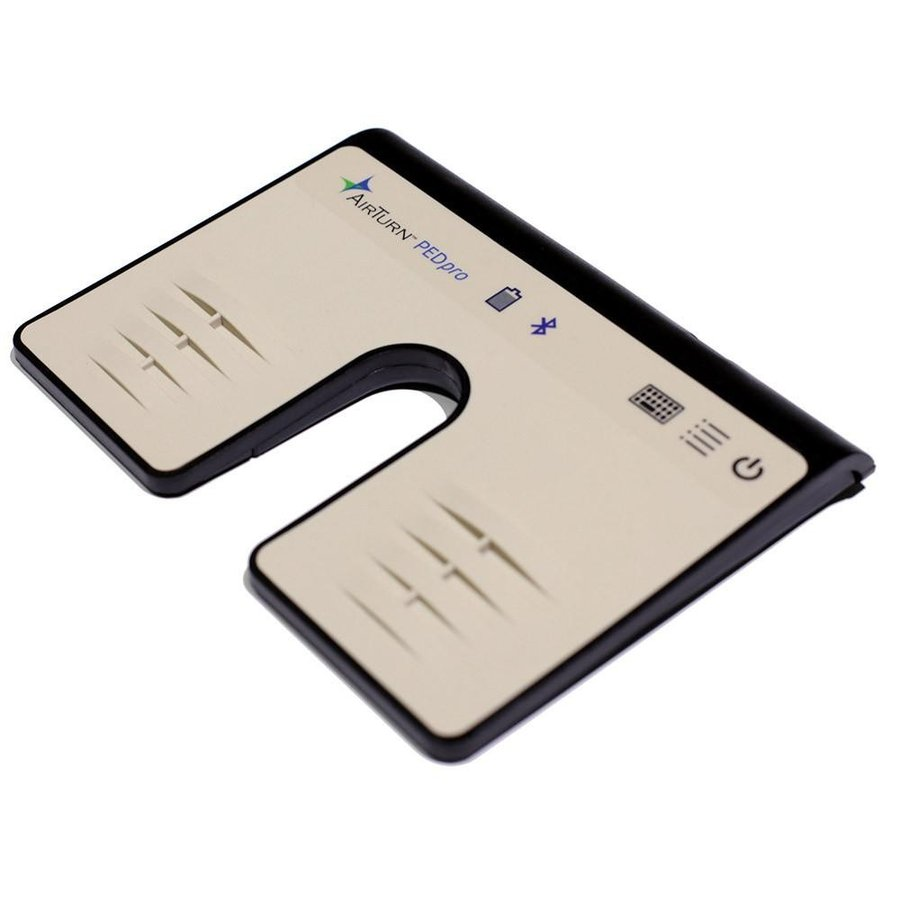
\includegraphics[width=40mm,bb=0 0 900 900]{figures/8d4f811f5a0c393acaff304102ba963f.jpg}}
\caption{A foot switch for turning a music score.}
\label{footswitch}
\end{figure}

%
% Good thing is that many keyboard devices are available for personal computers,
% and we can use such devices for using Gear.
% ``Key-repeat'' feature is useful for fast scrolling of the menu.


\subsubsection{2-way lever}

We have also tried to use a paddle-like device for generating {\up} and {\down}.
Users can push the puddle to the right to generate {\up} and
left to generate {\down}.
Pressure sensors are installed on the puddle, and
many {\up}'s are generated when the user pushes the puddle strongly.

\begin{figure}[H]
  \centerline{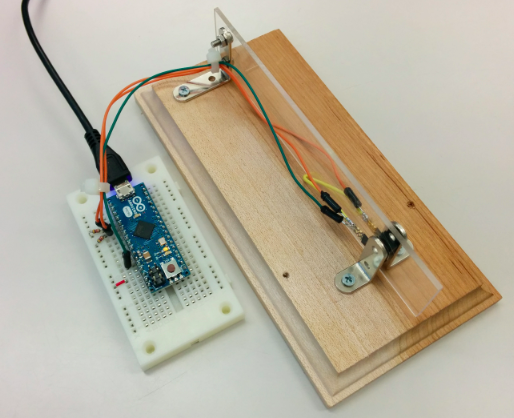
\includegraphics[width=54mm,bb=0 0 514 418]{figures/3c2de63899653056f3c6be835b9aaf43.png}}
\caption{Paddle device for Gear.}
\label{paddle}
\end{figure}

Controlling the speed of the scrolling of Gear by pressure is convenient,
since sometimes users want to jump to an entry far from current position.
That behavior is similar to the key-repeat feature of computer keyboards.

% Keys and pressure sensors can be placed anywhere:
% we tried putting two pressure sensors at the bottom of a chair, and it worked fine.

\subsubsection{Rotating devices}

We then tried various rotating devices for Gear.
%
We tried mouse wheels first, and found that they are very suitable for Gear,
because we are good at controlling our finger with precision.

Many kinds of rotating input devices have been used for controlling TVs and VCRs so far.
For example, ``jog dials'' have been widely used for controlling VCRs, and we tried the device for Gear.

\begin{figure}[H]
\centerline{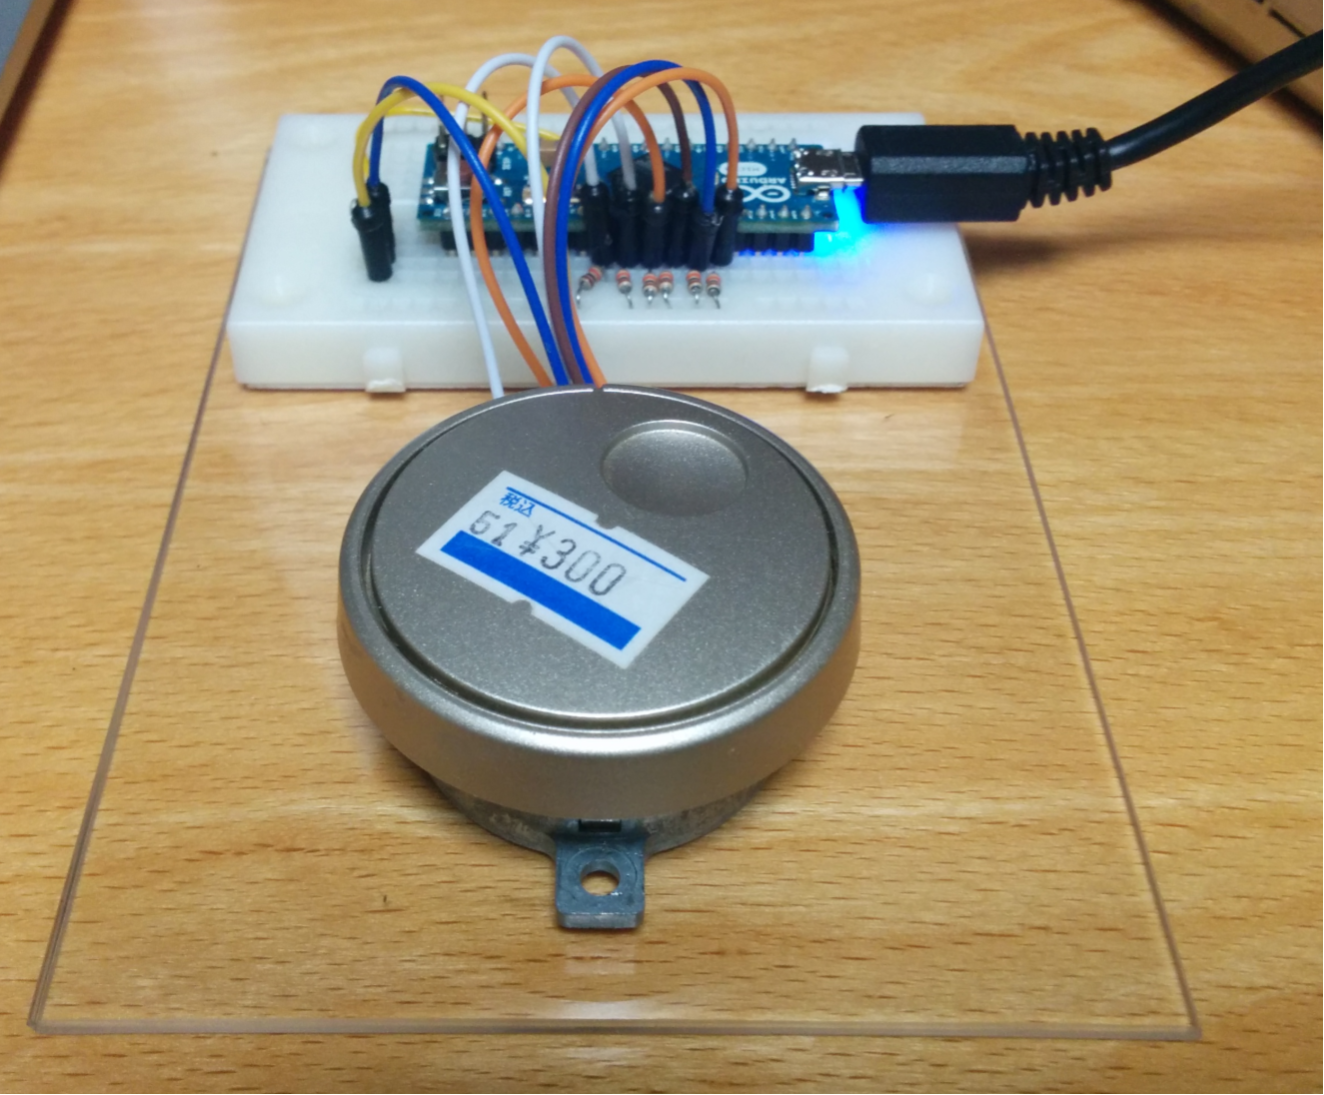
\includegraphics[width=54mm,bb=0 0 1324 1095]{figures/7a2c685b930cd30a267f4d564a8079be.png}}
\caption{Using a jog dial.}
\label{jog}
\end{figure}

\begin{figure}[H]
\centerline{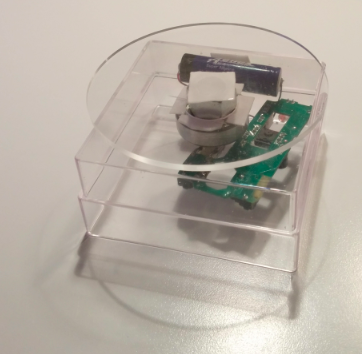
\includegraphics[width=54mm,bb=0 0 362 354]{figures/ff2d18e66f9a4655dbb5e22e0bb9a0ae.png}}
\caption{A disk-based device for Gear.}
\label{disk}
\end{figure}

We have also tried using a cylinder for Gear.
The rotating cylinder shown in Figure \ref{roller} is touching the mouse wheel, and
mouse wheel events are generated as the user rotates the cylinder using his arm or hand.

\begin{figure}[H]
\centerline{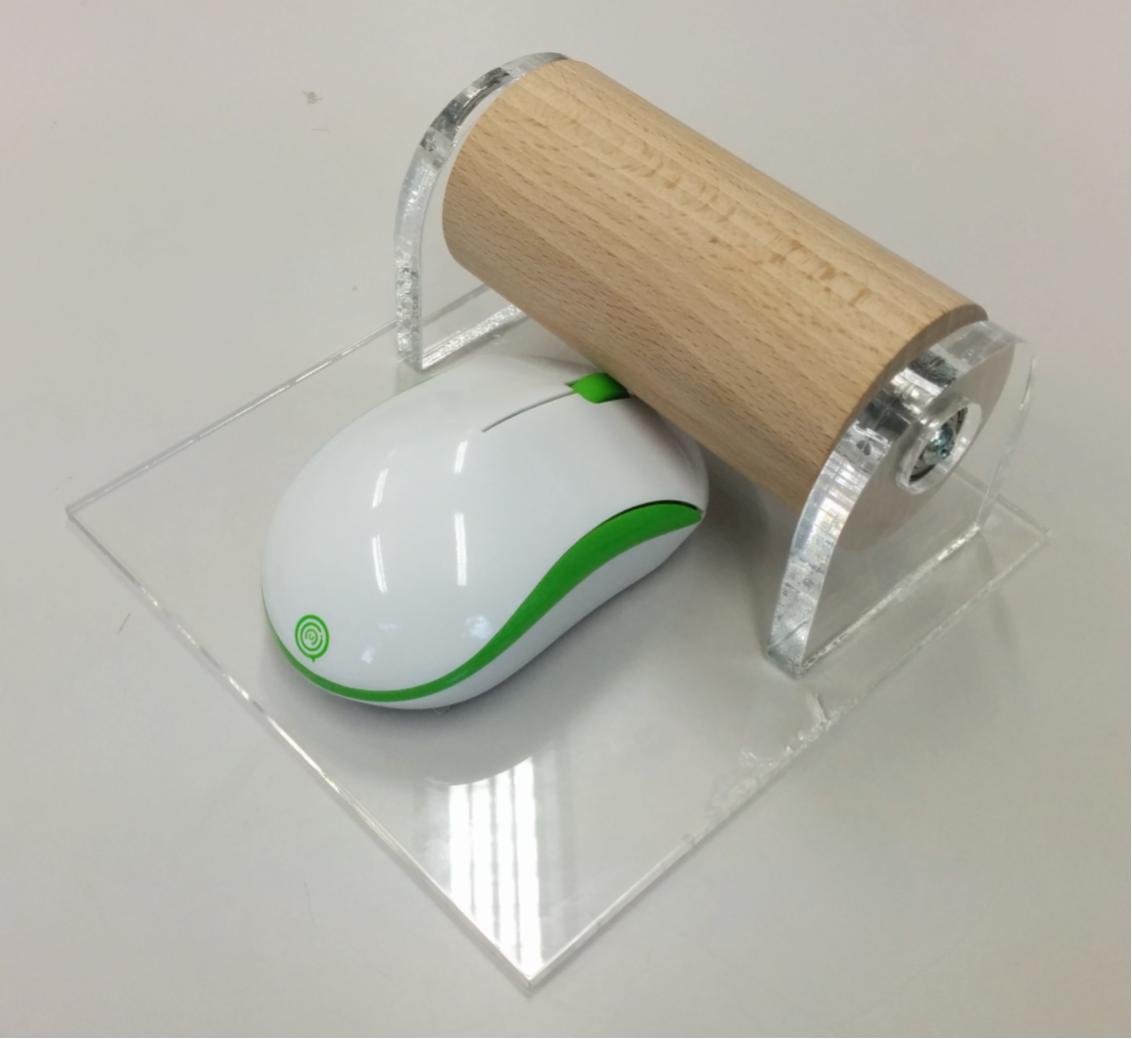
\includegraphics[width=54mm,bb=0 0 1132 1039]{figures/6ff91502ea4f3f3c47840c887148ada9.png}}
\caption{Using a roller.}
\label{roller}
\end{figure}

After trying these devices, we found that controlling rotating devices
like jog dials and cylinders are not as easy as we expected,
because precise control of an arm or a hand is fairly difficult.
People are good at controlling fingers, but people are usually not very good at
controlling arms and hands precisely.

% Keys and pressure sensors can be placed anywhere:
% we tried putting two pressure sensors at the bottom of a chair, and it worked fine.

\comment{
We tried a lever with two pressure sensors.
モールス用「エレキー」
Puddle

\begin{figure}[H]
\centerline{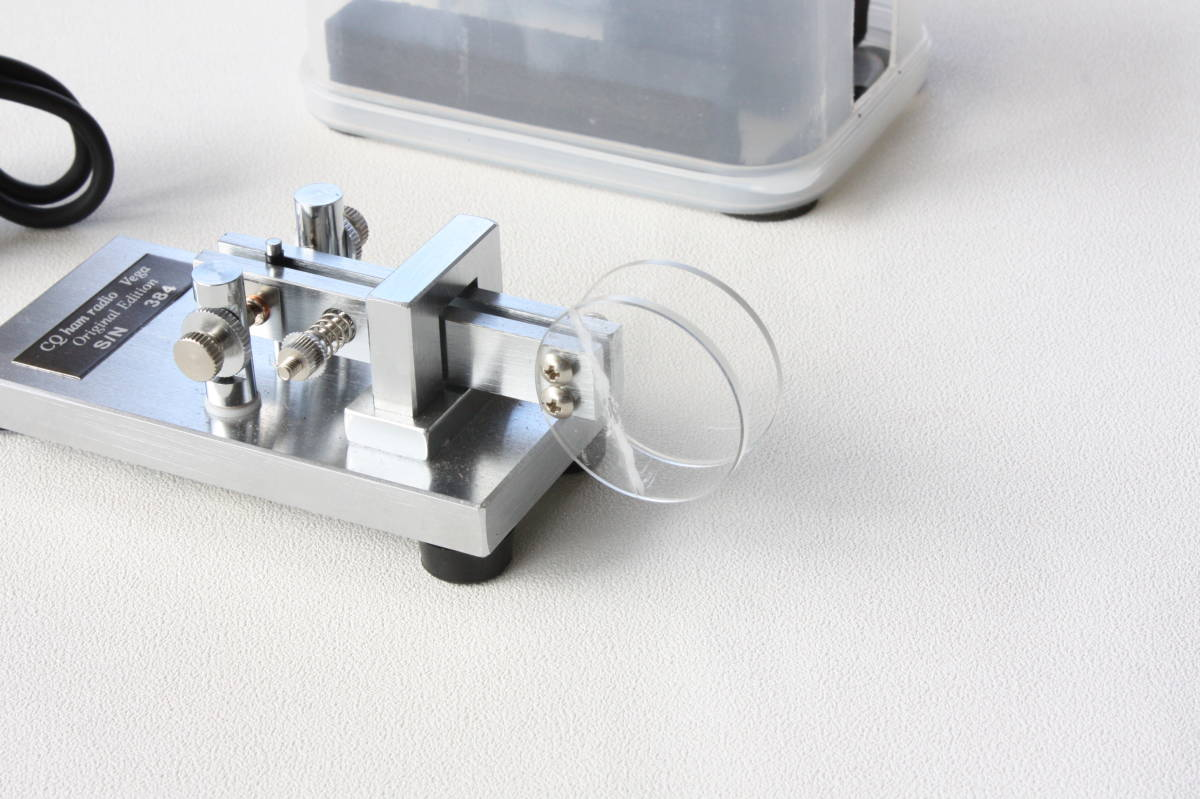
\includegraphics[width=80mm,bb=0 0 1200 799]{figures/d64d2a8e1dddc57f693267f811510f23.jpg}}
\caption{Elekey.}
\label{elekey}
\end{figure}
}

After trying various devices, it became clear that simple buttons or
wheels can be put at anywhere like on the table or under a chair, and
we felt that the integration of furniture and input devices will be
important in the IoT age.
%
If we can install the devices neatly on furniture and beds, people with disabilities can easily use them, 

\subsection{Comparison with existing navigation methods}

To compare the speed of Gear with conventional navigation method,
we created two applications for checking how fast a user can select an entry
from a large hierarchical database.
%
Both applications behaves the same way:
a user can set the date to a specific time to see a photo in a 15-minute monorail trip.
%
Using the first one (App1), a user can set the time using Gear (Figure \ref{monorailgear})
with up/down arrow keys for {\up} and {\down}.

\begin{figure}[H]
\centerline{
%  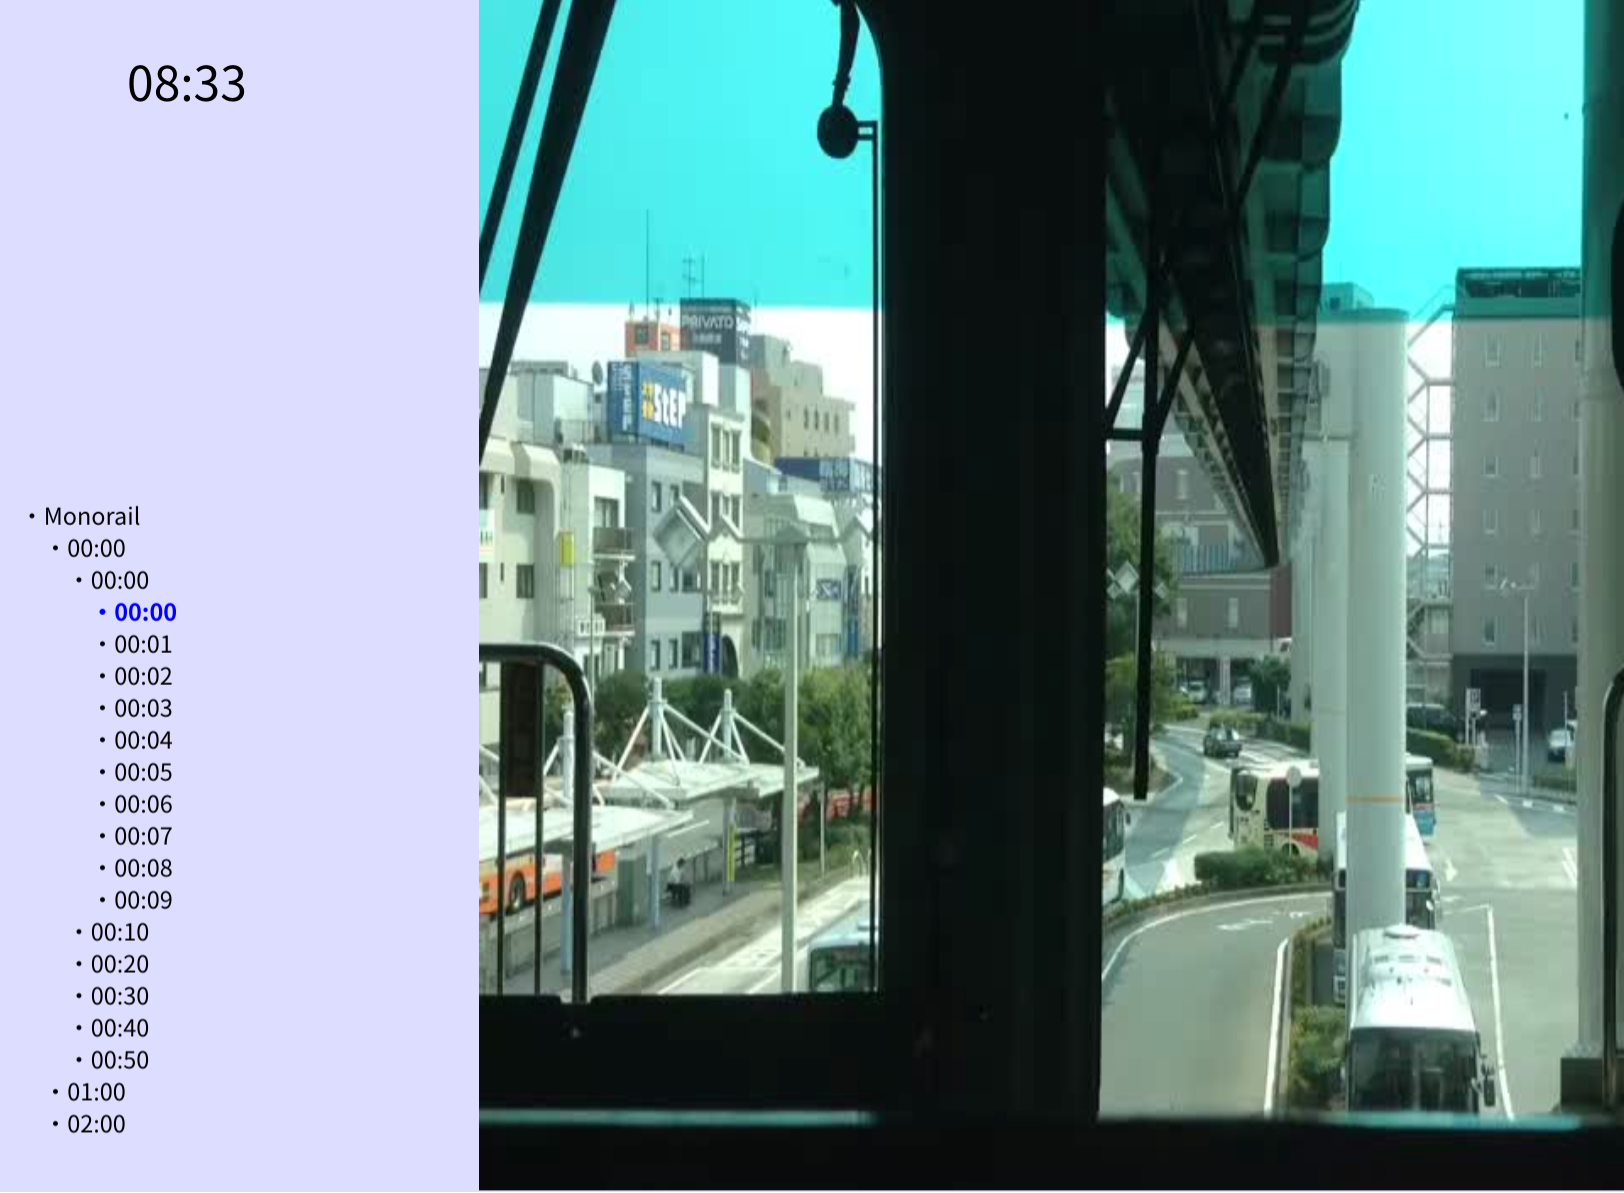
\includegraphics[width=38mm,bb=0 0 1624 1193]{figures/d663e8556732d40e70e55592ca1f1258.png}
  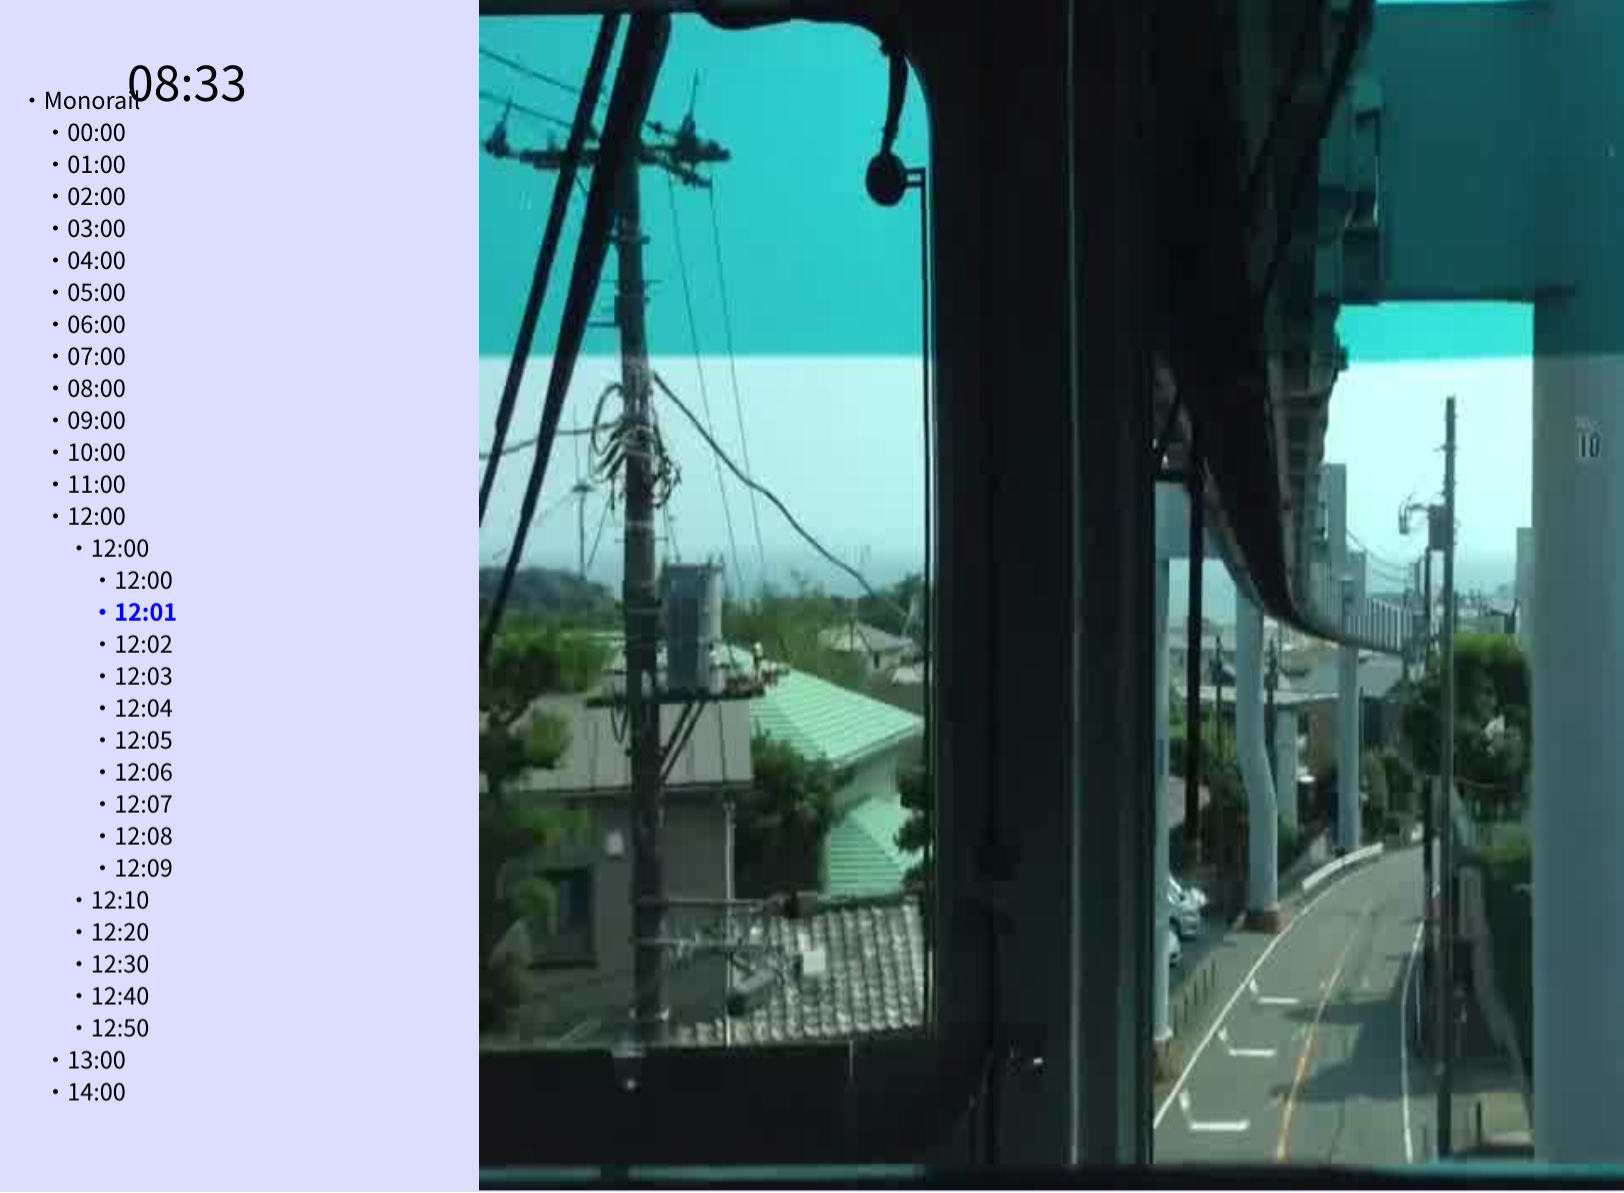
\includegraphics[width=70mm,bb=0 0 1624 1193]{figures/75007628f75ef1038bd5737e10a728b7.png}
}
\caption{App1: Gear-based application for finding a monorail picture.}
\label{monorailgear}
\end{figure}

Using the second one, a user can set the time using the \ttt{{\textless}input type="time"{\textgreater}} tag of HTML (Figure \ref{monorailinput}).
Users can first set the value of the ``minute'' value at the top-left using up/down cursor keys,
and move to the right with the right-arrow key and set the ``second'' value with up/down arrow keys.

\begin{figure}[H]
\centerline{
  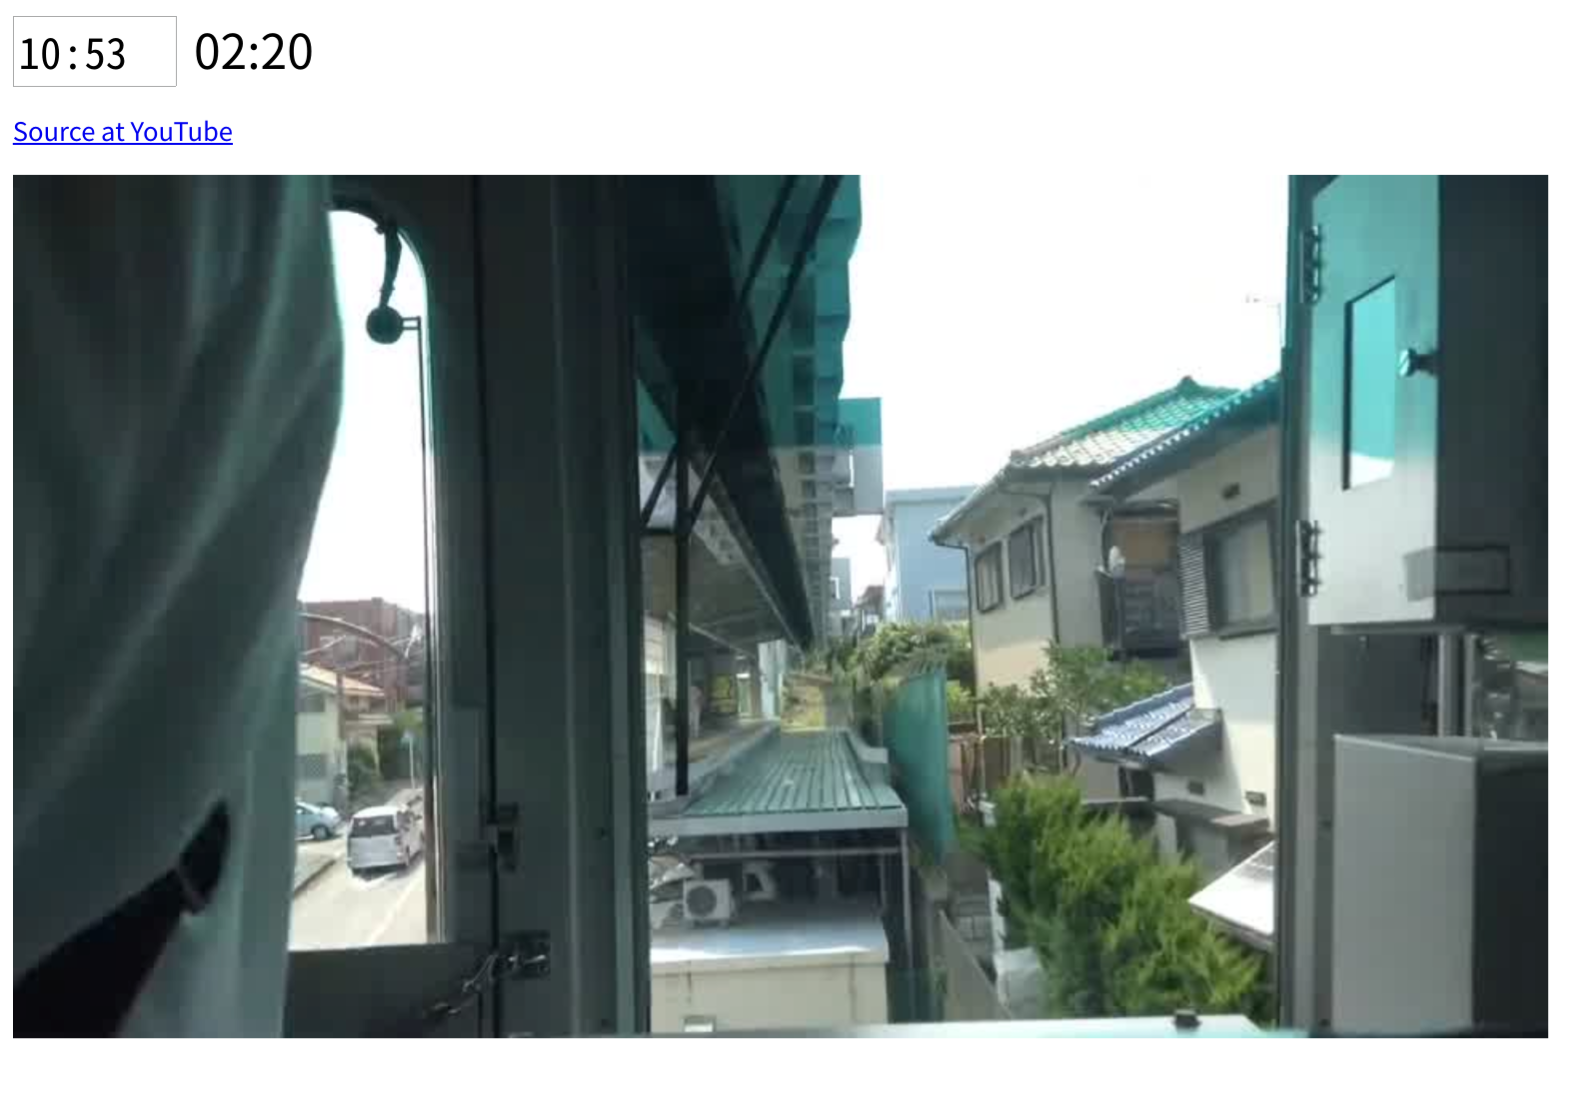
\includegraphics[width=70mm,bb=0 0 1596 1116]{figures/325208a6d94c68e4f08e61a67df419c4.png}
}
\caption{App2: using input element.}
\label{monorailinput}
\end{figure}

On both applications, a random target time is displayed on the screen and the subjects are
asked to set the time to the displayed target time.
After repeating the task 5 times, the average time is shown to the user, and the value
is reported.

We asked 5 people to try these tasks 10 times, and the result of the experiment is
shown in Figure \ref{monorailtime}.

\begin{figure}[H]
\centerline{
  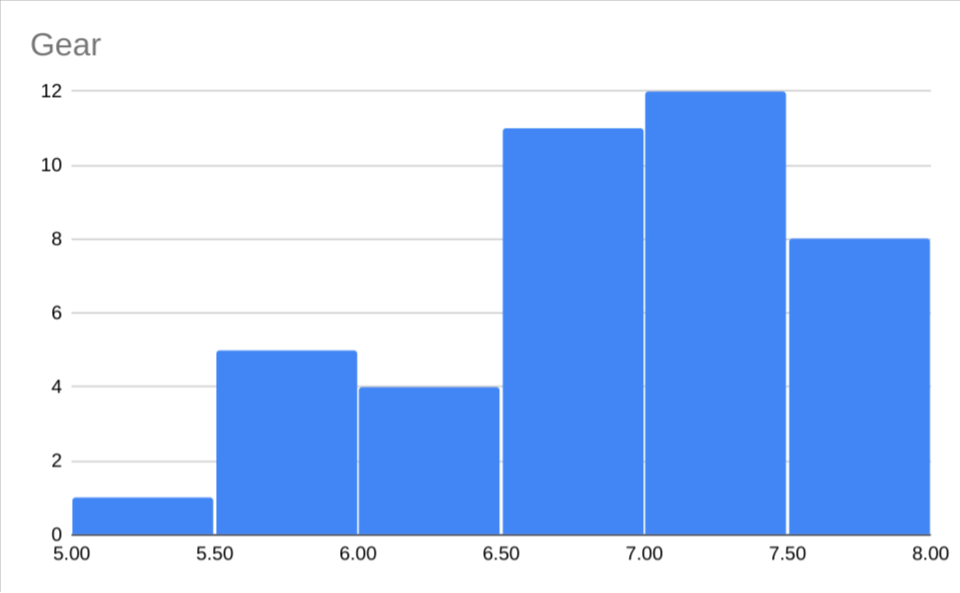
\includegraphics[width=38mm,bb=0 0 960 593]{figures/6c39f199b341e30ffc28850afbd90a5a.png}
  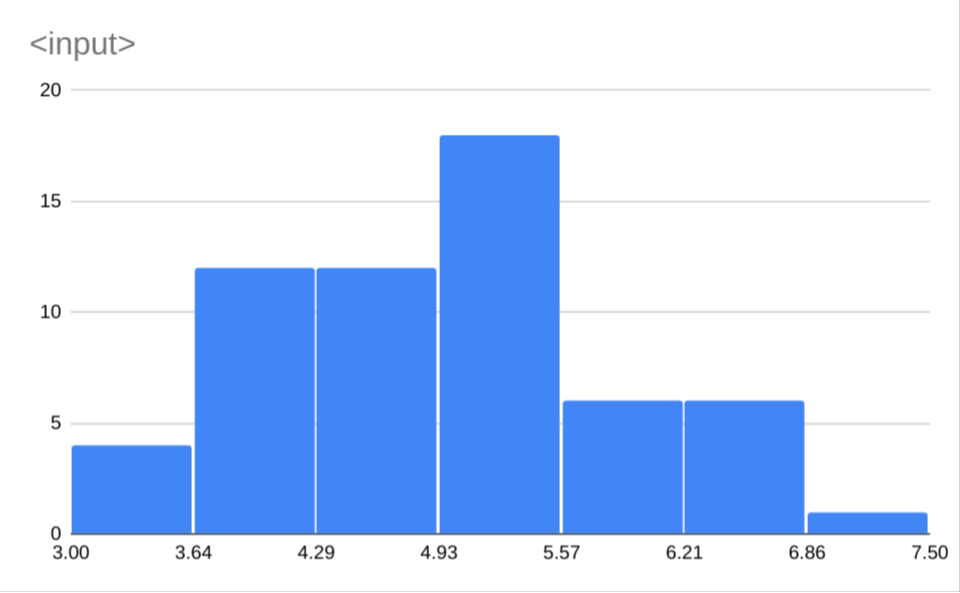
\includegraphics[width=38mm,bb=0 0 960 593]{figures/de3f0545e0d0d8dfb9708d2420fb5407.png}
}
\caption{Average search time of App1 and App2.}
\label{monorailtime}
\end{figure}

The average time for finding an entry using Gear was 6.84s,
and the average time using standard \ttt{{\textless}input{\textgreater}} was 4.96s.
It takes about 40\% more time than using conventional method.
The standard deviations were 0.71s and 0.93s, respectively.
%
This is a little bit disappointing,
but we are happy to see that
no-click browsing with Gear is not too slower than
conventional methods.

We have also tried using Finder.app for the same data (Figure \ref{noclickfinder}), and
got similar results as App2.

\comment{
4-way navigation is commonly used for exploring hierarchical data structure,
and it is familiar to computer users.
Some mobile phones and PDAs are equipped with a jog dial with a push button,
where the dial is used for choosing an item from the list and 
the push button is used for fixing the selection.
% PowerMate is equipped with a push button which can used for such purposes.
% As far as we know,
All the existing methods require more than 2 keys/buttons, and
to the best of the authors' knowledge,
Gear is the only interaction method for exploring hierarchical data structure
with one rotating device.
}

Using a conventional hierarchical menu,
child elements are displayed automatically when their parent element is selected by a mouse.
The behavior is well understood by computer users,
and Gear's automatic transition (e.g. from Figure \ref{fig4} to Figure \ref{fig5})
looks familiar to users.

\subsection{Comparison with InfoVis techniques}

Various information visualization techniques like
Treemap\cite{Johnson:1991:TSA:949607.949654},
Hyperbolic Tree\cite{Lamping:1995:FTB:223904.223956},
and Sunburst\cite{Stasko:2000:FDN:857190.857683}
have been proposed for visualizing large hierarchical data.
Zooming user interface (ZUI) systems like
Pad\cite{Perlin:1993:PAA:166117.166125} and
Pad++\cite{Bederson:1994:PZG:192426.192435}
can also be used for handling large hierarchical data laid out in a 2D space.
%
These visualization techniques and descendent technologies have become popular these days and
all of these systems are useful for understanding the structure of
large hierarchical data.
However, users of these systems have to use a pointing device
to take full advantage of these methods, and
no-click browsing is not supported.

% More conventional visualization techniques like TreeView\footnote{
%   \textsf{http://en.wikipedia.org/wiki/Tree\_view}
% } by replacing 4-way navigation to our approach.

% {\ST} can be adopted to more conventional visualization techniques like
% TreeView\footnote{
%   \textsf{http://en.wikipedia.org/wiki/Tree\_view}
% } by replacing 4-way navigation to our approach.

It seems to be a good idea to use Gear on more conventional visualization techniques like
TreeView\footnote{
  \textsf{http://en.wikipedia.org/wiki/Tree\_view}
}, by replacing 4-way navigation with Gear.

\begin{figure}[H]
\centerline{
  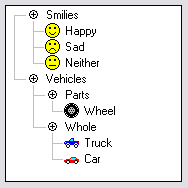
\includegraphics[width=38mm,bb=0 0 188 188]{figures/treeview.png}
}
\caption{A TreeView example.}
\label{treeview}
\end{figure}

% LensBar\cite{Masui:1998:LVB:647341.721215}
% is also a ZUI system for handling large hierarchical data,
% but the same data structure used in LensBar can be used for Gear.
% Users can use a pointing devices when it is appropriate,
% and use two keys or a disk device when pointing devices is not available.

\subsection{Timing control}

The biggest disadvantage of Gear is that
the behavior of Gear depends on the speed of the user's operations.
In Figure \ref{fig4},
if a user wanted to select \tsf{Clothing} but couldn't issue {\down}
quickly enough, he will see Figure \ref{fig5} instead of Figure \ref{fig7}.
This is a tradeoff between usability and simplicity, and
the best parameter should be set based on the user and the Gear device.

\subsection{Is the Gear interface new?}

Since the idea of Gear interface is so simple,
we have been wondering if the same idea existed in the past.
%
We could not find a research paper on 
navigation techniques based on two keys.
Many key-based navigation techniques are found on patent database,
but we could not find a navigation method based on two keys.
We are almost sure that The Gear interface had never been popular before.

\subsection{Using Gear in the wild}

One of the authors have been using Gear in his living room for several years
with a small personal computer connected to a 60-inch TV monitor.
The database is managed on {\SB}, and
a mouse wheel of a wireless Bluetooth mouse is used for Gear interface.
With Gear, the user can enjoy all available contents on the web with the mouse wheel
without selecting the source of the movies, animes, and musics from Amazon, Netflix, etc.

We can enjoy using Gear everywhere using a stick PC and a wireless mouse,
just like Amazon FireTV can be used for the same purpose.
Using {\SC} is more fun for the author, since no-click browsing is more comfortable than
selection-based interface on existing systems.

\comment{
Large dictionary database can also be treated as a large
hierarchical data, since the name of the entry can be treated hierarchically:
e.g. an entry for ``\tsf{dictionary}'' can be stored under ``\tsf{d}'', ``\tsf{d/i}'', and so on.

No formal evaluation have been done yet, but Gear has been used in the author's
living room for six months, and the author's family members are using it
everyday for watching anime films and listening to music.
Besides PowerMate, a wireless mouse is also used,
since we can carry it anywhere and select
a film or a music just by rotating the mouse wheel.
}

We demonstrated Gear at an exhibition
% held in November 2013,
and asked more than 100 people to try it
(Figure \ref{exhibition}).
%
Since the only thing a user can do with Gear was to rotate a wheel,
users seemed to be able to understand the behavior of Gear with trials and errors.
% 
% a user can use the device and see what happens without thinking about
% other interactions.
% 
Using only one rotating device for data navigation is a new experience for
all the visitors, but the hard restriction of the device seemed to have worked in this case.

\begin{figure}[H]
\centerline{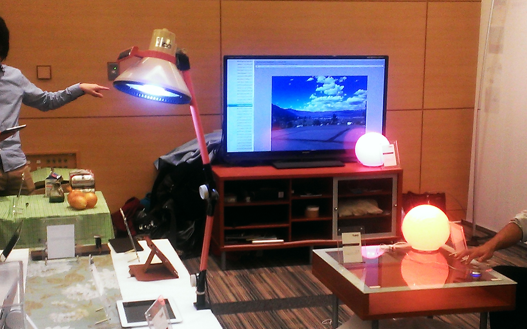
\includegraphics[width=84mm,bb=0 0 527 329]{figures/c520d5dfbd06c532d48d324a7019b00c.png}}
\caption{People at the right using a wheel device at an exhibition.}
\label{exhibition}
\end{figure}

% Selecting a content only by rotating a dial is very 気持ち良い。
% 音楽ソース、ニュースソース、動画、Wikipediaなどあらゆるものをダイヤルやペダルだけで検索できる

\section{Conclusion}

We have developed a new simple interaction method ``Gear'' for exploring
large hierarchical data structure.
A Gear user can easily find an entry in a huge hierarchical database
only by using a rotating input device which can be installed at
wide range of locations where conventional keyboards and switches do not fit.
We are hoping to install various implementations of Gear and try them at
various places like kitchens, restrooms, etc.

\small{
\bibliographystyle{IEEEtran}
\bibliography{paper}
}

\end{document}

